\PassOptionsToPackage{quiet}{fontspec}
\documentclass[12pt,a4paper,UTF8]{article}
\usepackage{thesis} % 格式控制
\usepackage{indentfirst}
\usepackage{amsmath} % 数学公式支持
\usepackage{amsfonts} % 数学字体支持
\usepackage{amssymb} % 数学符号支持
\usepackage{graphicx} % 图片插入支持
\usepackage{float} % 浮动体位置控制，支持 [H] 选项
\usepackage{caption} % 图表标题格式控制
\usepackage{geometry} % 页面布局控制
\usepackage{setspace} % 行距控制
\usepackage{xeCJK} % 中文字体支持
\usepackage{fontspec} % 字体设置
\usepackage[most]{tcolorbox} % 高亮按键命令
\usepackage{xcolor} % 颜色支持
\setlength{\parindent}{2em} % 控制首行缩进  
\addtolength{\parskip}{3pt} % 控制段落距离  
\onehalfspacing % 1.5倍行距  
\graphicspath{{./figures/}} % 指定图片所在文件夹  
\setCJKmainfont{SimSun}
% 定义中文字体命令
\setCJKfamilyfont{hei}{SimHei} 

\classname{天线理论与设计}  % 设置课程名称
\makepagestyle{}{\printclassname ~实验报告}

% 自定义命令
\newtcbox{\keyblue}{on line,
  colframe=blue!60!black, colback=blue!10,
  boxrule=0.8pt, arc=2pt, boxsep=0pt, left=2pt, right=2pt, top=1pt, bottom=1pt,
  tcbox raise base, fontupper=\color{blue}\bfseries}

\begin{document}
\maketitlepage{HFSS微带贴片天线设计与仿真}{玉泉教4-302}{郑智瑄}{3230103913}{\today}{王浩刚} %封面页 

\maketoc    %目录页

\section{实验原理}

微带天线是在一种薄的介质基板上，一面附上某种金属层作为接地板，另一面用蚀刻的方法可制成某种需要的形状，利用微带线或者同轴线等馈电方式馈电的天线形式。

如图 \ref{fig:microstrip} 所示，假设辐射贴片的长度近似为半波长，宽度为 w，介质基片的厚度为 h，天线的工作波长为 $\lambda$。

当我们把辐射贴片、介质基片和接地板视作一段长度为 $0.5\lambda$ 的低阻抗传输线，且传输线的两端形成开路。由于介质基片的厚度远远小于波长，所以电场的强度在厚度这一方向基本保持不变。

在最简单的情况下，我们同样假设电场强度沿着宽度 w 方向也没有变化。那么，在只考虑主模激励的（TM10 模）的情况下，该天线的电场结构如图 \ref{fig:sideview} 所示，辐射基本是可以认为是由辐射贴片开路边的边缘引起的。

在两开路端的电场可以分解为相对于接地板的水平分量和垂直分量。由于辐射贴片长度约为半个波长，因此两开路端电场的垂直分量方向相反，水平分量方向相同。所以，两开路端的水平分量电场可以等效为无限大平面上同相激励的两个缝隙，缝隙的宽度为 $\Delta L$，长度为 w，两缝隙间距为半波长，缝隙的电场沿着 w 方向均匀分布，电场垂直于 w 方向。

    \begin{figure}[H]
        \centering
        \begin{minipage}[b]{0.45\linewidth}
            \centering
            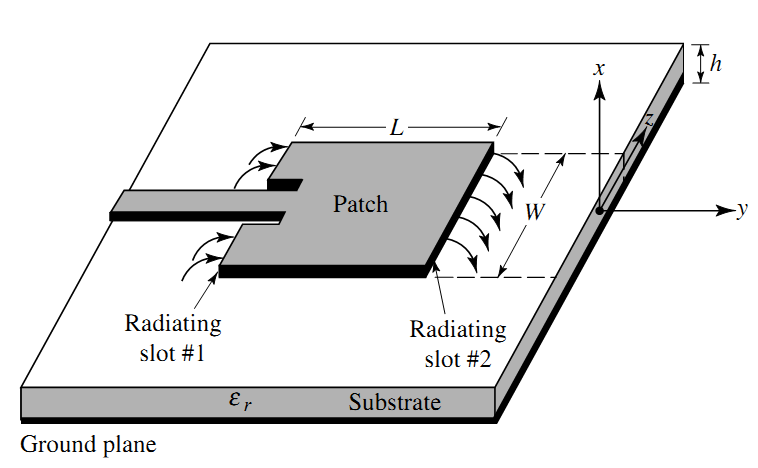
\includegraphics[width=0.9\textwidth]{e1.png}
            \caption{矩形微带天线结构}
            \label{fig:microstrip}
             
        \end{minipage}%
        \begin{minipage}[b]{0.45\linewidth}
            \centering
            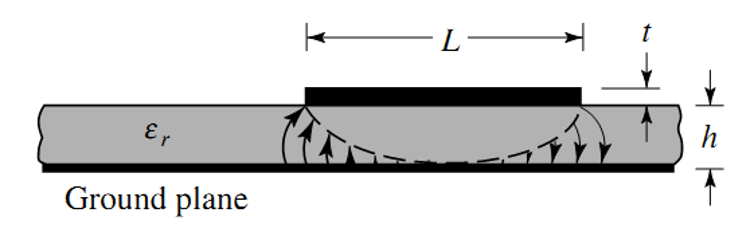
\includegraphics[width=0.9\textwidth]{e2.png}
            \caption{侧视图}
            \label{fig:sideview}
             
        \end{minipage}
    \end{figure}

\clearpage
\section{天线参数计算}

由设计要求，天线的中心频率 $f_r = 10GHz$，介质基片的相对介电常数 $\epsilon_r = 10.2$，高度 $h = 0.05 in = 0.127 cm$。

\subsection{辐射贴片的宽度 W 计算}

宽度 $W$ 使用以下公式计算：
$$ W = \frac{c}{2f_r}\sqrt{\frac{2}{\epsilon_r+1}} $$

其中 $c = 3\times10^{10}$ cm/s，$f_r = 10$ GHz $= 10\times10^9$ Hz。代入数据，得：

$$ W  \approx 0.6339 \text{ cm} $$

进而得 $\frac{W}{h} = \frac{0.6339}{0.127} \approx 4.991$。

\subsection{辐射贴片长度 L 计算}

\subsubsection{计算有效介电常数 $\epsilon_{eff}$}

贴片天线的 $\epsilon_{eff}$ 可以用微带线的公式来近似。由于 $\frac{W}{h} \approx 4.991 > 1$，代入有效相对介电常数公式：

$$ \epsilon_{eff} = \frac{\epsilon_r+1}{2} + \frac{\epsilon_r-1}{2}\left(1+12\frac{h}{W}\right)^{-0.5} $$

求得

$$ \epsilon_{eff} \approx 8.093 $$

\subsubsection{计算有效长度 $L_{eff}$}

贴片在 $L$ 方向上谐振，其有效长度 $L_{eff}$ 为半个导波长 $\lambda_g/2$：

$$ L_{eff} = \frac{\lambda_g}{2} = \frac{\lambda_0}{2\sqrt{\epsilon_{eff}}} = \frac{c}{2f_r\sqrt{\epsilon_{eff}}} $$

求得

$$ L_{eff} \approx 0.5273 \text{ cm} $$

\subsubsection{计算边缘效应长度 $\Delta L$}

边缘场效应使得贴片的电长度比物理长度长。这个增量 $\Delta L$ 可以通过以下经验公式计算：

$$ \Delta L = 0.412h \frac{(\epsilon_{eff}+0.3)(\frac{W}{h}+0.264)}{(\epsilon_{eff}-0.258)(\frac{W}{h}+0.8)} $$

代入已知值 $\epsilon_{eff} \approx 8.093$，$\frac{W}{h} \approx 4.991$ 和 $h = 0.127$ cm

求得，

$$ \Delta L = 0.05232 \times 0.9721 \approx 0.0509 \text{ cm} $$

\subsubsection{计算物理长度 $L$}

物理长度 $L$ 是有效长度减去两端的边缘效应增量：

$$ L = L_{eff} - 2\Delta L = 0.5273 - 2\times 0.0509 = 0.5273 - 0.1018 $$

故

$$L = \frac{\lambda}{2} - 2\Delta L = \frac{c}{2f_r\sqrt{\epsilon_{eff}}} - 2\Delta L \approx 0.4255 \text{ cm}$$

\subsection{微带线宽度 $W_0$ 计算}

又该天线与特性阻抗为 $50\Omega$ 的微带线相连，由 Eq 14-19 可知：

假设 $\frac{W_0}{h} \leq 1$，由
$$ Z_c = \begin{cases}
\frac{60}{\sqrt{\epsilon_{eff}}} \ln(\frac{8h}{W_0} + \frac{W_0}{4h}), & \frac{W_0}{h} \leq 1 \\
\frac{120\pi}{\sqrt{\epsilon_{eff}}[\frac{W_0}{h}+1.393+0.667\ln(\frac{W_0}{h}+1.444)]}, & \frac{W_0}{h} > 1
\end{cases} $$

其中 $Z_c = 50\Omega$，即可解得此微带线的宽度为 $W_0 = 0.76h = 0.0966 cm$，满足假设。

\subsection{馈线嵌入距离 $y_0$ 计算}

与此同时，设辐射点和辐射贴片边缘的距离为 $y_0$。由于 $\lambda_0 = \frac{c}{f_r} = 3 cm > W = 0.6339 cm$，有 $G_1 = \frac{1}{90}(\frac{W}{\lambda})^2 = 4.96\times10^{-4} Siemens$，又由 Eq 14-18a，求得 $G_{12} = 4.079\times10^{-4} Siemens$，故可得 $Z_{in} = \frac{1}{2(G_1+G_{12})} = 553.16\Omega$。

选择输入阻抗为 $50\Omega$ 的馈点，有：$50 = Z_{in}\cos^2(\frac{\pi}{L}y_0)$，即可解得：
$$ y_0 = \frac{1.265}{\pi}L = 0.1713 cm $$

即馈线嵌入距离 $y_0 = 0.1713 cm$。

\subsection{切缝宽度 $d_0$ 计算}

切缝的主要作用是调整输入阻抗，改善阻抗匹配性能。根据经验法则，切缝宽度应在 $0.2W_0 \sim 0.5W_0$ 范围内，即 $0.0193 cm \sim 0.0483 cm$。
在此先取$d_0 = 0.045 cm = 0.45 mm$

\subsection{天线参数汇总}

综合上述计算，微带贴片天线的所有设计参数汇总如表 \ref{tab:antenna_parameters} 所示。

\begin{table}[H]
\centering
\caption{微带贴片天线设计参数汇总}
\label{tab:antenna_parameters}
\begin{tabular}{cccc}
\hline
\textbf{变量} & \textbf{参数名称} & \textbf{取值} & \textbf{单位} \\
\hline
$f_r$ & 中心频率 & 10 & GHz \\
$c$ & 光速 & $3\times10^{10}$ & cm/s \\
$\epsilon_r$ & 相对介电常数 & 10.2 & - \\
$h$ & 介质基片高度 & 0.127 & cm \\
$\lambda_0$ & 自由空间波长 & 3.00 & cm \\
\hline
$W$ & 辐射贴片宽度 & 0.6339 & cm \\
$\frac{W}{h}$ & 宽高比 & 4.991 & - \\
$\epsilon_{eff}$ & 有效介电常数 & 8.093 & - \\
$L_{eff}$ & 有效长度 & 0.5273 & cm \\
$\Delta L$ & 边缘效应长度 & 0.0509 & cm \\
$L$ & 辐射贴片物理长度 & 0.4255 & cm \\
\hline
$Z_c$ & 微带线特性阻抗 & 50 & $\Omega$ \\
$W_0$ & 50$\Omega$微带线宽度 & 0.0966 & cm \\
\hline
$y_0$ & 馈线嵌入距离 & 0.1713 & cm \\
\hline
$d_0$ & 切缝宽度 & 0.045 & cm \\
\hline
\end{tabular}
\end{table}

\clearpage
\section{仿真步骤}

\subsection{工程初始化}

\begin{enumerate}
    \item 运行 HFSS 软件并新建工程，将工程文件另存为 Microstrip.aedt。
    \item 设置求解类型，在主菜单栏中选择 \keyblue{HFSS}—\keyblue{Solution Type}，在弹出窗口中选择 \keyblue{Modal}，单击 \keyblue{OK}，完成设置。
    \item 设置模型长度单位，在主菜单栏中选择 \keyblue{Modeler}—\keyblue{Units}，选择 \keyblue{cm}。
\end{enumerate}

\subsection{变量设定}

在主菜单栏中选择 \keyblue{HFSS}—\keyblue{Design Properties}，打开涉及属性对话框，单击 \keyblue{add} 按钮，打开 \keyblue{AddProperty} 对话框，添加设计变量，如下图：

\begin{figure}[H]
    \centering
    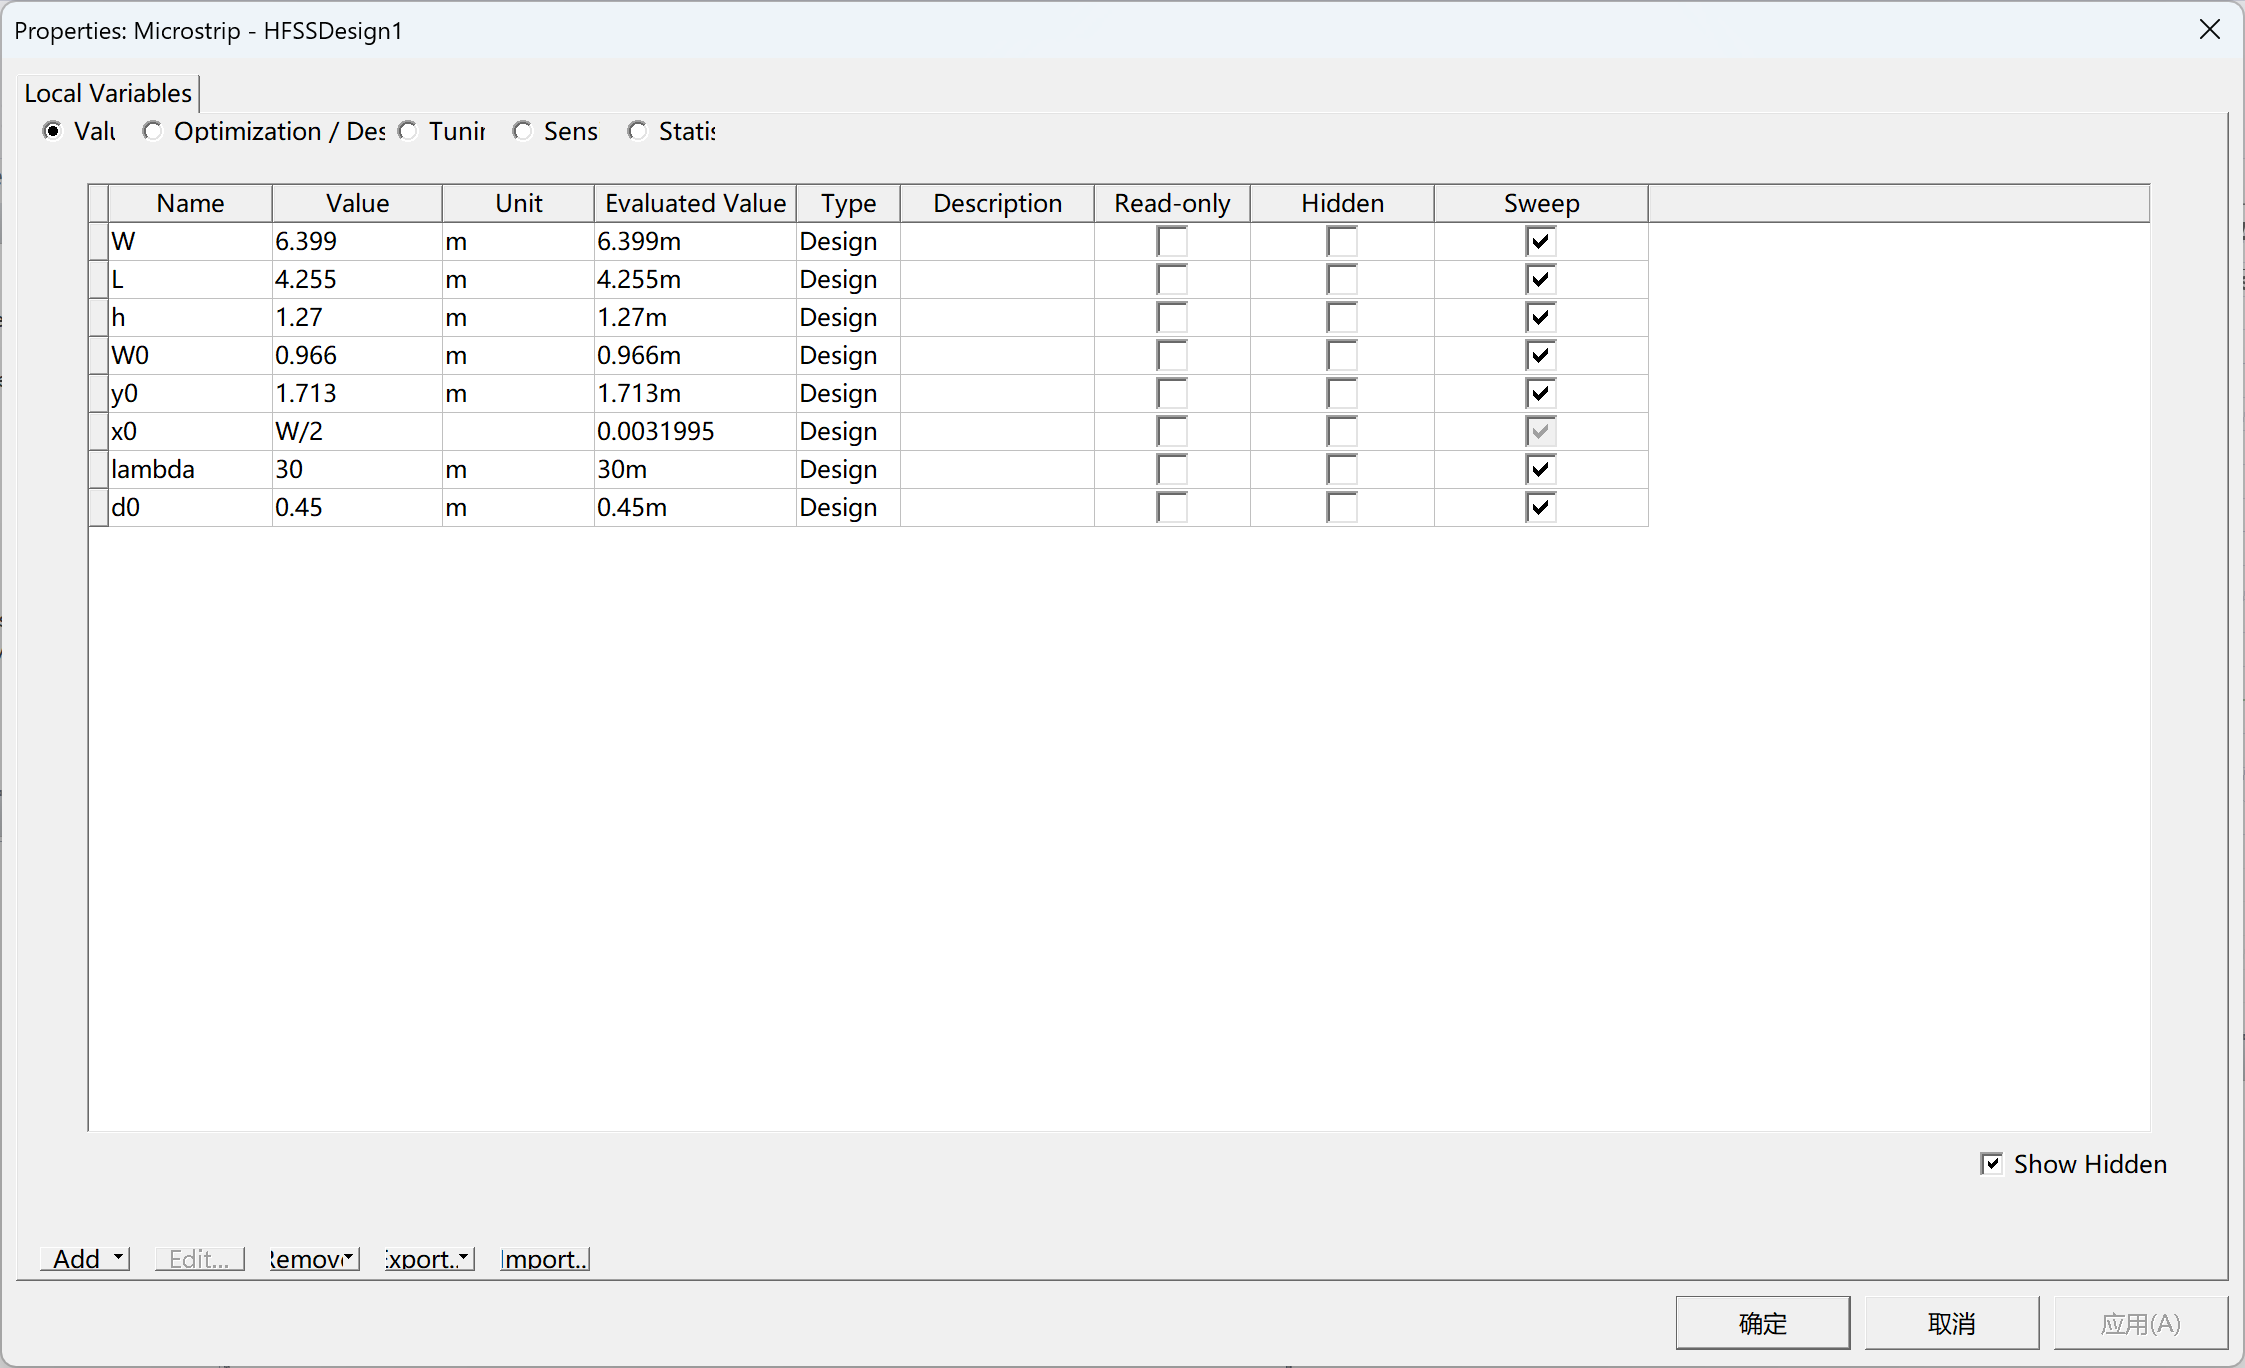
\includegraphics[width=0.8\textwidth]{p1.png}
    \caption{添加和定义设计变量}
    \label{fig:design_properties}
\end{figure}

\subsection{天线建模}

总的来说，微带天线一共包含有四个部分：{\heiti 介质基片}、{\heiti 辐射贴片}、{\heiti 四分之一波长阻抗转换器}、{\heiti 50$\Omega$ 微带传输线}。其可以在 HFSS 中使用长方体或矩形面进行绘制。对于 PEC 材质的贴片和地面，我们可以通过给一个二维平面模型分配理想导体边界条件的方式进行模拟。为便于观察，我们以 $x$ 轴作为 $L$ 的方向，以 $y$ 轴作为 $W$ 的方向，各部分的设计建模流程如下：

\subsubsection{介质基片建模}

在 HFSS 中，我们需要绘制长方体作为介质基片。针对此次仿真的天线，其介质基片的相对介电常数为 10.2，尺寸为 $5L \times 5W \times h$，底面为地面、材质为 PEC，仿真步骤如下：

\begin{enumerate}
    \item 在主菜单栏中选择 \keyblue{Draw}—\keyblue{Box} 或单击工具栏上的长方体按钮，进入创建长方体的状态。新建的长方体会添加到操作历史树的 \keyblue{Solids} 节点下，默认名为 \keyblue{Box1}。
    
    \item 双击操作历史树中 \keyblue{Solids} 下的 \keyblue{Box1} 节点，将长方体名称设置为 \keyblue{Substrate}，新增材质属命名为 \keyblue{Sub}，且在其 \keyblue{Relative Permittivity} 一栏中填写 10.2，损耗角正切设为 0.003（更符合实际材料）。
    
    \item 双击操作历史树中 \keyblue{Substrate} 下的 \keyblue{CreateBox} 节点，打开新建长方体属性对话框的 \keyblue{Command} 选项卡，在选项卡中设置长方体的底面顶点坐标、长、宽、高。在 \keyblue{Position} 文本框中输入底面顶点坐标 \texttt{(-5*L/2, -5*W/2, 0)}，在 \keyblue{XSize} 文本框中输入长度值 \texttt{5*L}，在 \keyblue{YSize} 文本框中输入宽度值 \texttt{5*W}，在 \keyblue{ZSize} 文本框中输入高度值 \texttt{h}，点击确定，完成介质基片 \keyblue{Substrate} 的创建。
    
    \item 选中 \keyblue{Substrate} 的下表面，单击右键，在菜单中选择 \keyblue{Edit}—\keyblue{Surface}—\keyblue{Create Object From Face}，从而新建地面。其会添加到操作历史树的 \keyblue{Sheets} 节点下，默认名为 \keyblue{Substrate\_ObjectFromFace1}。
    
    \item 双击 \keyblue{Substrate\_ObjectFromFace1} 节点，将矩形名称设置为 \keyblue{GND}，点击确定。
    
    \item 右键单击操作历史树中的 \keyblue{GND} 节点，选择 \keyblue{Assign Boundary}—\keyblue{Perfect E}，将该平面设置为完美电导体，点击确定，完成地面的创建。
\end{enumerate}

\subsubsection{辐射贴片建模}

在 HFSS 中，我们使用矩形面作为天线的辐射贴片。针对此次仿真的天线，其辐射贴片材质为 PEC，尺寸为 $L \times W$，仿真步骤如下：

\begin{enumerate}
    \item 在主菜单栏中选择 \keyblue{Draw}—\keyblue{Rectangle} 或单击工具栏上的矩形按钮，进入创建矩形的状态。新建的矩形会添加到操作历史树的 \keyblue{Sheets} 节点下，默认名为 \keyblue{Rectangle1}。
    
    \item 双击操作历史树中 \keyblue{Sheets} 下的 \keyblue{Rectangle1} 节点，将矩形名称设置为 \keyblue{Patch}，点击确定。
    
    \item 双击操作历史树中 \keyblue{Patch} 下的 \keyblue{CreateRectangle} 节点，打开新建矩形属性对话框的 \keyblue{Command} 选项卡，在选项卡中设置矩形的顶点坐标、长和宽。在 \keyblue{Position} 文本框中输入顶点坐标 \texttt{(-L/2, -W/2, h)}，在 \keyblue{XSize} 文本框中输入长度值 \texttt{L}，在 \keyblue{YSize} 文本框中输入宽度值 \texttt{W}，点击确定，完成辐射贴片 \keyblue{Patch} 的创建。
\end{enumerate}

\subsubsection{四分之一波长阻抗转换器建模}

同理，该部分使用矩形面作为天线的用阻抗作为 1/4 波长阻抗转换器，其仿真步骤如下：

\begin{enumerate}
    \item 在主菜单栏中选择 \keyblue{Draw}—\keyblue{Rectangle} 或单击工具栏上的矩形按钮，进入创建矩形的状态。新建的矩形会添加到操作历史树的 \keyblue{Sheets} 节点下，默认名为 \keyblue{Rectangle1}。
    
    \item 双击操作历史树中 \keyblue{Sheets} 下的 \keyblue{Rectangle1} 节点，将矩形名称设置为 \keyblue{Transition}，点击确定。
    
    \item 双击操作历史树中 \keyblue{Transition} 下的 \keyblue{CreateRectangle} 节点，打开新建矩形属性对话框的 \keyblue{Command} 选项卡，在选项卡中设置矩形的顶点坐标、长和宽。在 \keyblue{Position} 文本框中输入顶点坐标 \texttt{(L/2-y0, -W0/2, h)}，在 \keyblue{XSize} 文本框中输入长度值 \texttt{lambda/4}，在 \keyblue{YSize} 文本框中输入宽度值 \texttt{W0}，点击确定，完成四分之一波长阻抗转换器 \keyblue{Transition} 的创建。
\end{enumerate}

\subsubsection{50$\Omega$ 微带传输线建模}

在 HFSS 中，我们使用矩形面作为 50$\Omega$ 微带传输线，其仿真步骤如下：

\begin{enumerate}
    \item 在主菜单栏中选择 \keyblue{Draw}—\keyblue{Rectangle} 或单击工具栏上的矩形按钮，进入创建矩形的状态。新建的矩形会添加到操作历史树的 \keyblue{Sheets} 节点下，默认名为 \keyblue{Rectangle1}。
    
    \item 双击操作历史树中 \keyblue{Sheets} 下的 \keyblue{Rectangle1} 节点，将矩形名称设置为 \keyblue{Microstrip}，点击确定。
    
    \item 双击操作历史树中 \keyblue{Microstrip} 下的 \keyblue{CreateRectangle} 节点，打开新建矩形属性对话框的 \keyblue{Command} 选项卡，在选项卡中设置矩形的顶点坐标、长和宽。在 \keyblue{Position} 文本框中输入顶点坐标 \texttt{(L/2-y0+lambda/4, -W0/2, h)}，在 \keyblue{XSize} 文本框中输入长度值 \texttt{5*L/2-(L/2-y0+lambda/4)}，在 \keyblue{YSize} 文本框中输入宽度值 \texttt{W0}，点击确定，完成 50$\Omega$ 微带传输线的创建。
\end{enumerate}

\subsubsection{矩形面合并与切缝生成}

\begin{enumerate}
    \item 按住 \keyblue{Ctrl} 键，依次单击工程树 \keyblue{Sheets} 节点下的 \keyblue{Patch}、\keyblue{Transition}、\keyblue{Microstrip} 三个矩形面，再选择主菜单中的 \keyblue{Modeler}—\keyblue{Boolean}—\keyblue{Unite} 命令，执行合并操作，使即可合并成一个完整金属片与最先创建的矩形面即 \keyblue{Patch} 相同。
    
    \item 右键单击操作历史树中的 \keyblue{Patch} 节点，选择 \keyblue{Assign Boundary}—\keyblue{Perfect E}，将该平面设置为完美电导体，点击确定。
    
    \item 在主菜单栏中选择 \keyblue{Draw}—\keyblue{Rectangle} 或单击工具栏上的矩形按钮，进入创建矩形的状态。新建的矩形会添加到操作历史树的 \keyblue{Sheets} 节点下，默认名为 \keyblue{Rectangle1}。
    
    \item 双击操作历史树中 \keyblue{Sheets} 下的 \keyblue{Rectangle1} 节点，将矩形名称设置为 \keyblue{Cut1}，点击确定。
    
    \item 双击操作历史树中 \keyblue{Cut1} 下的 \keyblue{CreateRectangle} 节点，打开新建矩形属性对话框的 \keyblue{Command} 选项卡，在选项卡中设置矩形的顶点坐标、长和宽。在 \keyblue{Position} 文本框中输入顶点坐标 \texttt{(L/2-y0, -W0/2-d0, h)}，在 \keyblue{XSize} 文本框中输入长度值 \texttt{y0}，在 \keyblue{YSize} 文本框中输入宽度值 \texttt{W0}，点击确定。
    
    \item 同理，新建矩形 \keyblue{Cut2}，与 \keyblue{Cut1} 分别位于 1/4 波长阻抗转换器的两侧。其顶点坐标为 \texttt{(L/2-y0, W0/2, h)}，长为 \texttt{y0}，宽为 \texttt{d0}。
    
    \item 依次选中 \keyblue{Sheets} 节点下的 \keyblue{Patch}、\keyblue{Cut1}、\keyblue{Cut2}，再选择主菜单中的 \keyblue{Modeler}—\keyblue{Boolean}—\keyblue{Subtract} 命令，执行数剪操作，此时绘制得到的微带天线如图 \ref{fig:antenna_model} 所示。
\end{enumerate}

\begin{figure}[H]
    \centering
    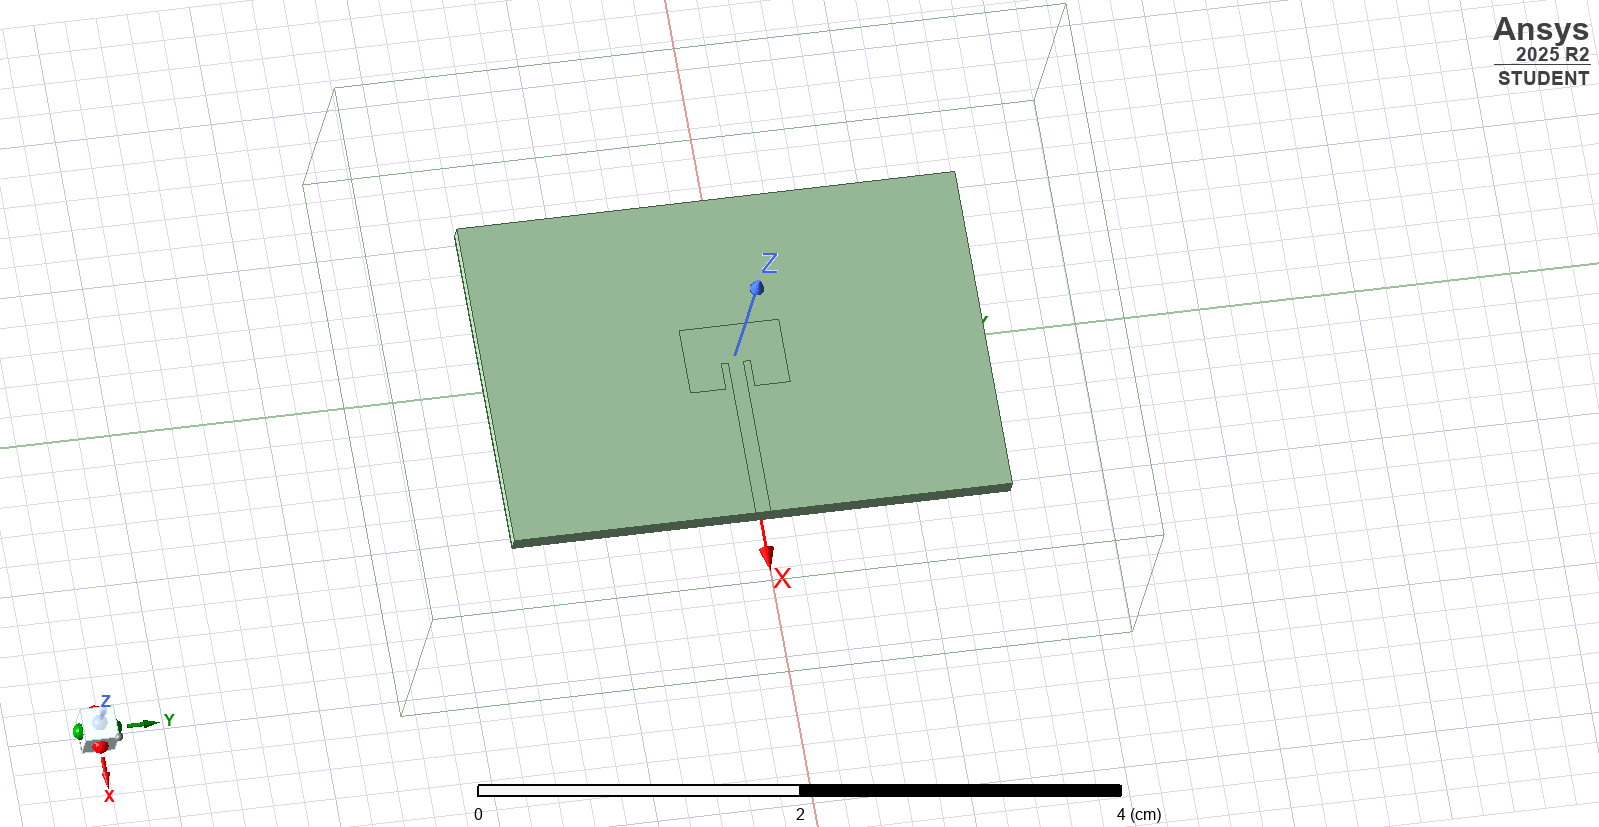
\includegraphics[width=0.8\textwidth]{p7.png}
    \caption{微带天线模型}
    \label{fig:antenna_model}
\end{figure}

\subsection{端口设置}

\subsubsection{设置辐射边界条件}

在 HFSS 中，辐射边界表面距离辐射体通常需要不小于 1/4 个工作波长，在 10GHz 的工作频率下即为 0.75 cm。在此次仿真中，我们使用长方体的表面作为辐射边界，其各个面与辐射贴片的距离均为 0.75 cm，仿真步骤如下：

\begin{enumerate}
    \item 在菜单栏中选择 \keyblue{Create Region}，并在弹出的窗口中将 \keyblue{Padding Type} 改为 \keyblue{Absolute Offset}，\keyblue{Value} 改为 \texttt{lambda/4}，点击 \keyblue{OK}。
    
    \item 双击操作历史树下 \keyblue{Solids} 的 \keyblue{Region} 节点，打开属性对话框，将区域材质改为 \keyblue{air}，透明度为 0.8，点击确定。
    
    \item 右键单击操作历史树中的 \keyblue{Region} 节点，选择 \keyblue{Assign Boundary}—\keyblue{Radiation}，在弹出的对话框中保留默认设置，从而将长方体的表面设置为辐射边界。
\end{enumerate}

\subsubsection{设置端口激励}

在此次仿真中，传输线终端使用集总端口激励。集总端口平面宽度设置为微带线宽度，高度设置为介质基片高度，端口底面和参考地相连，并使端口负载为 50$\Omega$，仿真步骤如下：

\begin{enumerate}
    \item 在工具栏上的 \keyblue{XY} 下拉菜单列表框，选择 \keyblue{YZ} 选项，将当前工作面设置为 \texttt{yz} 平面。
    
    \item 在主菜单栏中选择 \keyblue{Draw}—\keyblue{Rectangle} 或单击工具栏上的矩形按钮，进入创建矩形的状态。新建的矩形会添加到操作历史树的 \keyblue{Sheets} 节点下，默认名为 \keyblue{Rectangle1}。
    
    \item 双击操作历史树中 \keyblue{Sheets} 下的 \keyblue{Rectangle1} 节点，将矩形名称设置为 \keyblue{Port}，点击确定。
    
    \item 双击操作历史树中 \keyblue{Port} 下的 \keyblue{CreateRectangle} 节点，打开新建矩形属性对话框的 \keyblue{Command} 选项卡，在选项卡中设置矩形的顶点坐标、长和宽。在 \keyblue{Position} 文本框中输入顶点坐标 \texttt{(5*L/2, -W0/2, 0)}，在 \keyblue{YSize} 文本框中输入长度值 \texttt{W0}，在 \keyblue{ZSize} 文本框中输入宽度值 \texttt{h}，点击确定。
    
    \item 右键单击操作历史树中的 \keyblue{Port} 节点，选择 \keyblue{Assign Excitation}—\keyblue{Lumped Port}，在打开的集总端口数设置对话框中，将 \keyblue{Full Port Impedance} 设为 50$\Omega$，单击下一页。
    
    \item 在 \keyblue{Modes} 对话框中单击 \keyblue{Integration Line} 旁下的 \keyblue{None}，在主菜单中选择 \keyblue{Draw Lines} 命令，在 \keyblue{Port} 对话框中画出一条从下至上的端口积分线，在 \keyblue{Port Processing} 对话框中选择 \keyblue{Do Not Renormalize}，单击完成。
\end{enumerate}

\begin{figure}[H]
    \centering
    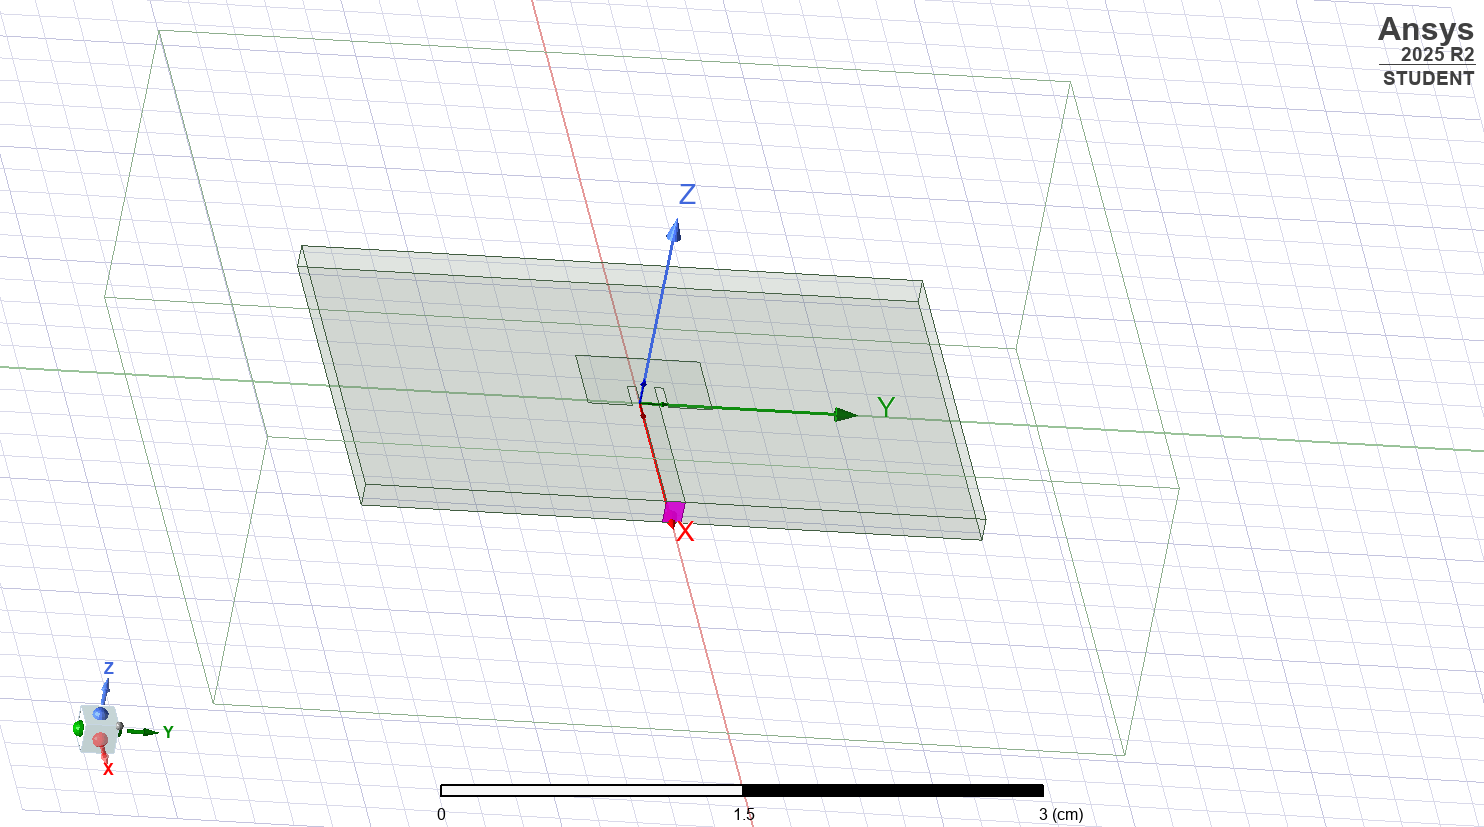
\includegraphics[width=0.5\textwidth]{p8.png}
    \caption{端口激励设置}
    \label{fig:port_Excitation}
\end{figure}

\subsection{求解设置}

\subsubsection{求解设置}

针对此次的微带天线，其中心频率为 10GHz，扫频范围是 8GHz -- 14GHz，因此求解频率范围设置为 8GHz -- 14GHz。插值扫描的输入阻抗与阻抗数据，具体步骤如下：

\begin{enumerate}
    \item 右键单击工程树下的 \keyblue{Analysis}，在弹出的对话框选中 \keyblue{Add Solution Setup}，将求解频率设置为 10GHz，自适应网格分的最大迭代次数设置为 20，收敛设差至 0.02。
    
    \item 展开工程树下的 \keyblue{Analysis} 节点，右键单击其扫描设置 \keyblue{Setup1}，在弹出的对话框选中 \keyblue{Add Frequency Sweep}，将扫描频率设置为快速扫描，扫频范围填写为 \texttt{8GHz -- 14GHz}，点数为 6000，点击确定。
\end{enumerate}

\subsubsection{设计检查和运行仿真}

在进行仿真设计，我们已经完成了模型的创建和解算设置等前期工作，在运行仿真之前，需要进行设计检查，确认设计的完整性和正确性，唯有 HFSS 设计完整无误，方可进行仿真计算，仿真步骤如下：

\begin{enumerate}
    \item 选择主菜单中的 \keyblue{HFSS}—\keyblue{Validation Check}，进行设计检查，若弹出的对话框中表示此次仿真，则表示此设计正确，可以进行下一步计算。
    
    \item 右键单击工程树下的 \keyblue{Analysis}—\keyblue{Setup1}，在弹出的菜单中选择 \keyblue{Analyze}，运行仿真计算。
\end{enumerate}

\section{仿真数据后处理与分析}

\subsection{回波损耗}

\begin{enumerate}
    \item 右键单击工程树下的 \keyblue{Results} 节点，在弹出的菜单中选择
    
    \keyblue{Create Model Solution Data Report}—\keyblue{Rectangle Plot} 命令，打开报告设置对话框。
    
    \item 依次在 \keyblue{Category}、\keyblue{Function} 中选择 \keyblue{S Parameter}、\keyblue{dB}，点击 \keyblue{New Report}，再单击 \keyblue{Close}，得到回波损耗结果报告如图 \ref{fig:s11} 所示。
\end{enumerate}

\begin{figure}[H]
    \centering
    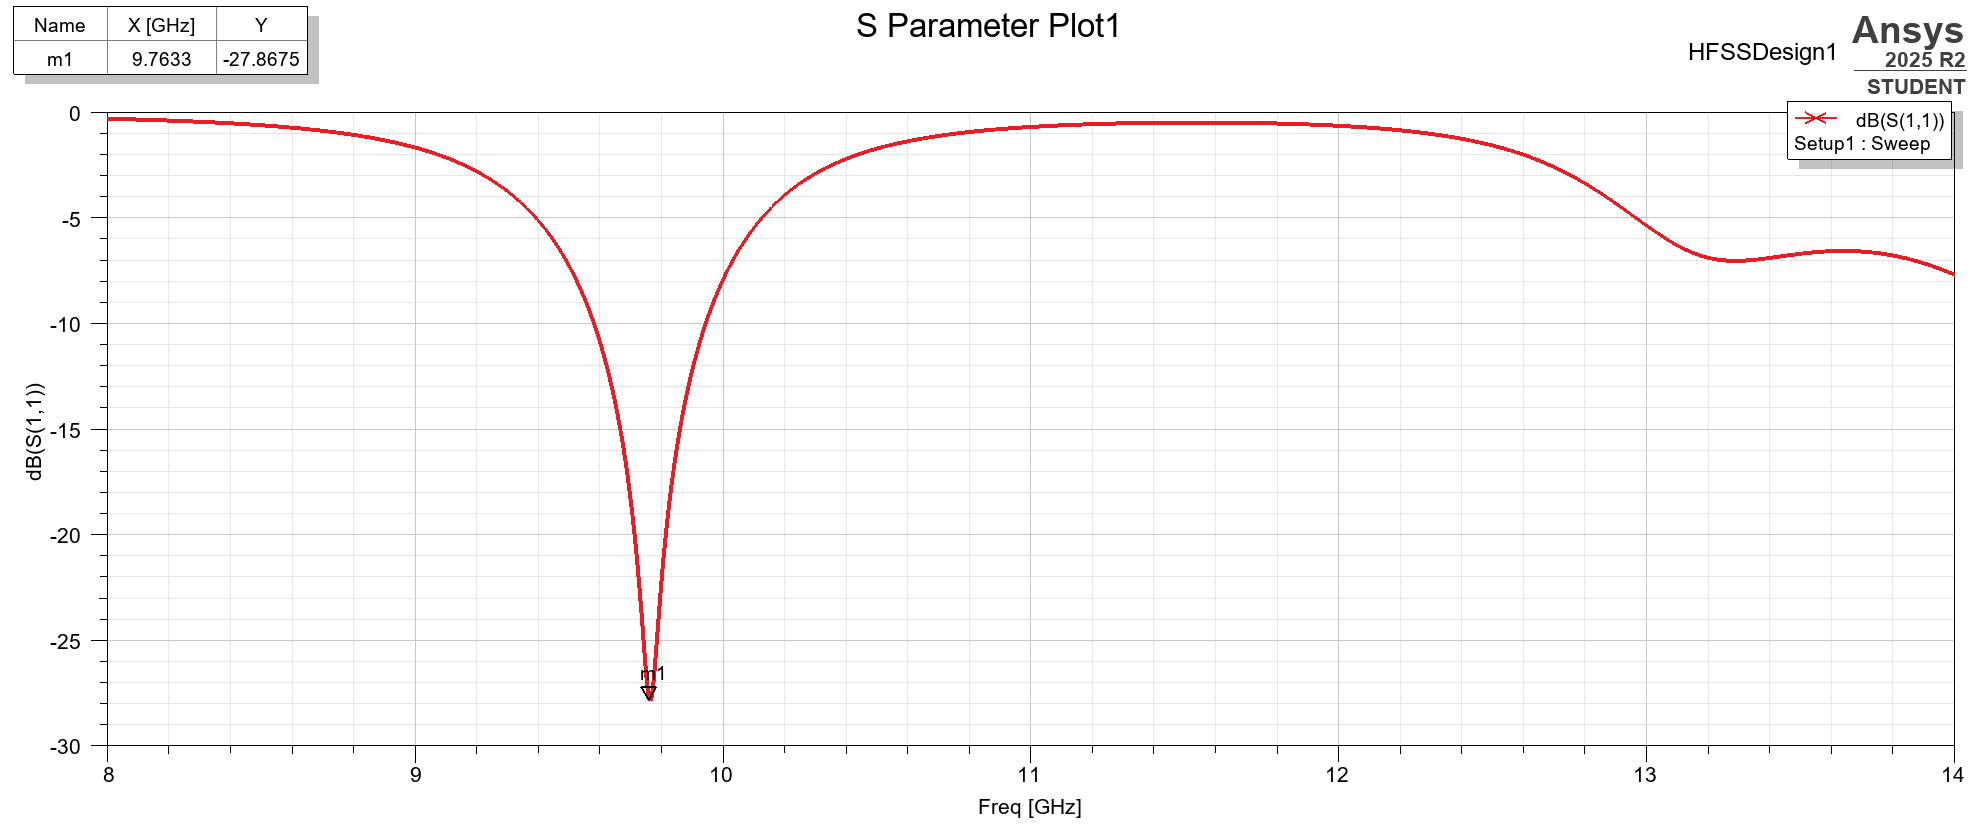
\includegraphics[width=1\textwidth]{p9.png}
    \caption{回波损耗}
    \label{fig:s11}
\end{figure}

【实验结果】:由仿真结果图 \ref{fig:s11}（回波损耗）可知：天线的谐振频率为 9.7633 GHz，此时的回波损耗（$S_{11}$）为 -27.8675 dB。该值远小于 -10 dB，表明天线在此频率下具有良好的阻抗匹配。
同时，-10dB带宽约为0.35GHz，工作频率范围约为9.58GHz至9.93GHz,在12GHz附近可见输入阻抗的高次模谐振峰。


\subsection{输入阻抗}

\begin{enumerate}
    \item 右键单击工程树下的 \keyblue{Results} 节点，在弹出的菜单中选择
    
    \keyblue{Create Model Solution Data Report}—\keyblue{Rectangle Plot} 命令，打开报告设置对话框。
    
    \item 依次在 \keyblue{Category}、\keyblue{Function} 中选择 \keyblue{Z Parameter}、\keyblue{im} 和 \keyblue{re}，点击 \keyblue{New Report}，再单击 \keyblue{Close}，得到天线的输入阻抗结果报告如图 \ref{fig:impedance} 所示。
\end{enumerate}

\begin{figure}[H]
    \centering
    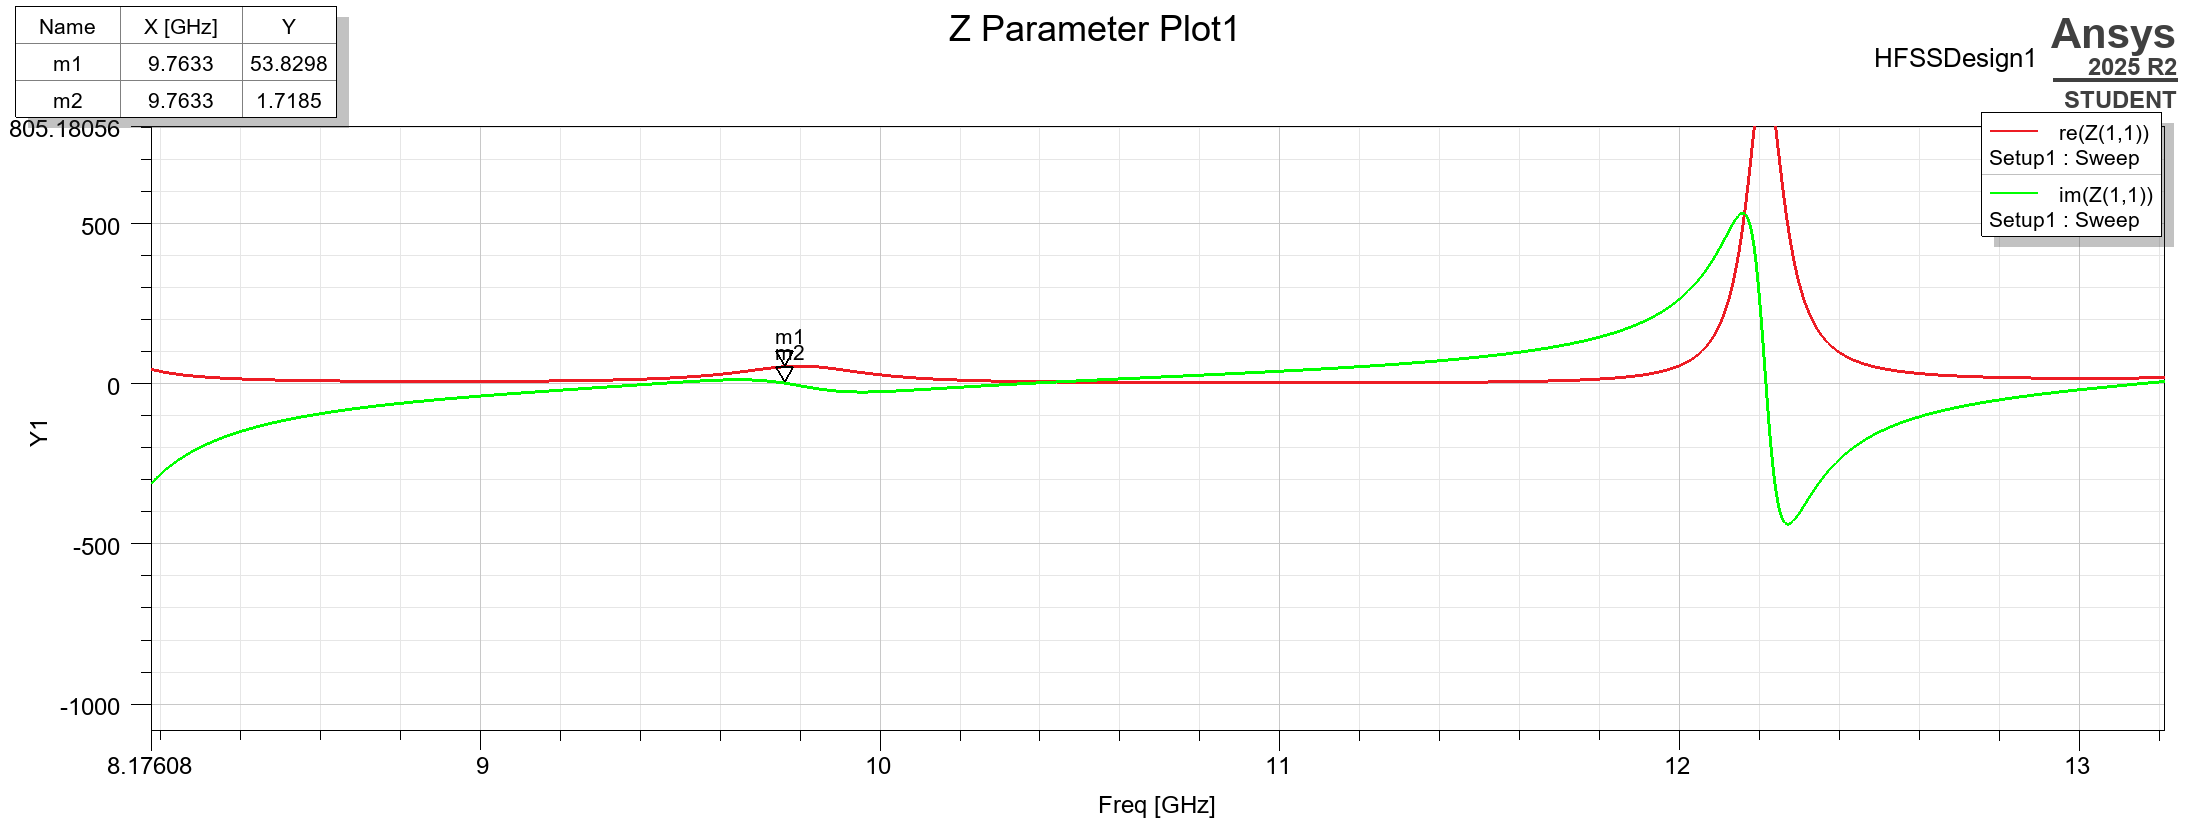
\includegraphics[width=1.0\textwidth]{p10.png}
    \caption{天线输入阻抗}
    \label{fig:impedance}
\end{figure}

【实验结果】：由仿真结果图 \ref{fig:impedance}（天线输入阻抗）可知：在谐振频率 9.7633 GHz 处，天线输入阻抗的实部为 53.8298 $\Omega$，虚部为 1.7185 $\Omega$。该阻抗值接近 50 $\Omega$ 的目标，与图 \ref{fig:s11} 的回波损耗结论一致。
同时，呈现了电阻偶对称、电抗奇对称的特征，和理论一致。

\subsection{方向图}

\subsubsection{方向图仿真设置}

为得到天线在 HFSS 谐振频率（$f_0 = 9.7633GHz$）下的方向图，需重新创建一个新的求解设置 \keyblue{Setup2}，其求解频率为 9.7633GHz，其余设置值与 \keyblue{Setup1} 一致，运行仿真计算。

首先定义辐射表面：

\begin{enumerate}
    \item 右键单击工程树下的 \keyblue{Radiation} 节点，在弹出的快速菜单中选择 \keyblue{Insert Far Field Setup}—\keyblue{Infinite Sphere}，打开 \keyblue{Far Radiation Sphere Setup}，在此处定义辐射表面。

    \item 定义辐射表面 \keyblue{E Plane}，其中，\keyblue{Phi} 的始末角度为 0$^\circ$，步长为 0；\keyblue{Theta} 从 -180$^\circ$ 到 180$^\circ$，步长为 1$^\circ$。

    \item 同理，定义辐射表面 \keyblue{H Plane}，其中，\keyblue{Phi} 的始末角度为 90$^\circ$，步长为 0；\keyblue{Theta} 从 -180$^\circ$ 到 180$^\circ$，步长为 1$^\circ$。

    \item 同理，定义辐射表面 \keyblue{3D Sphere}，其中，\keyblue{Phi} 从 0$^\circ$ 到 360$^\circ$，步长为 1$^\circ$；\keyblue{Theta} 从 0$^\circ$ 到 180$^\circ$，步长为 1$^\circ$。
\end{enumerate}

\subsubsection{E 平面方向图}

\begin{enumerate}
    \item 右键单击工程树下的 \keyblue{Results} 节点，在弹出的菜单中选择 \keyblue{Create Far Fields Report}—\keyblue{Radiation Pattern} 命令，打开报告设置对话框。
    
    \item 在对话框左侧 \keyblue{Solution} 中选择 \keyblue{Setup2}，\keyblue{Geometry} 中选择 \keyblue{E Plane}；右侧 \keyblue{Primary Sweep} 中选择 \keyblue{Theta}，下方 \keyblue{Category}、\keyblue{Quantity}、\keyblue{Function} 中依次选择 \keyblue{Gain}、\keyblue{GainTotal}、\keyblue{dB}，点击 \keyblue{New Report}，再单击 \keyblue{Close}，得到天线 E 平面的方向图如图 \ref{fig:e_plane} 所示。
\end{enumerate}

\begin{figure}[H]
    \centering
    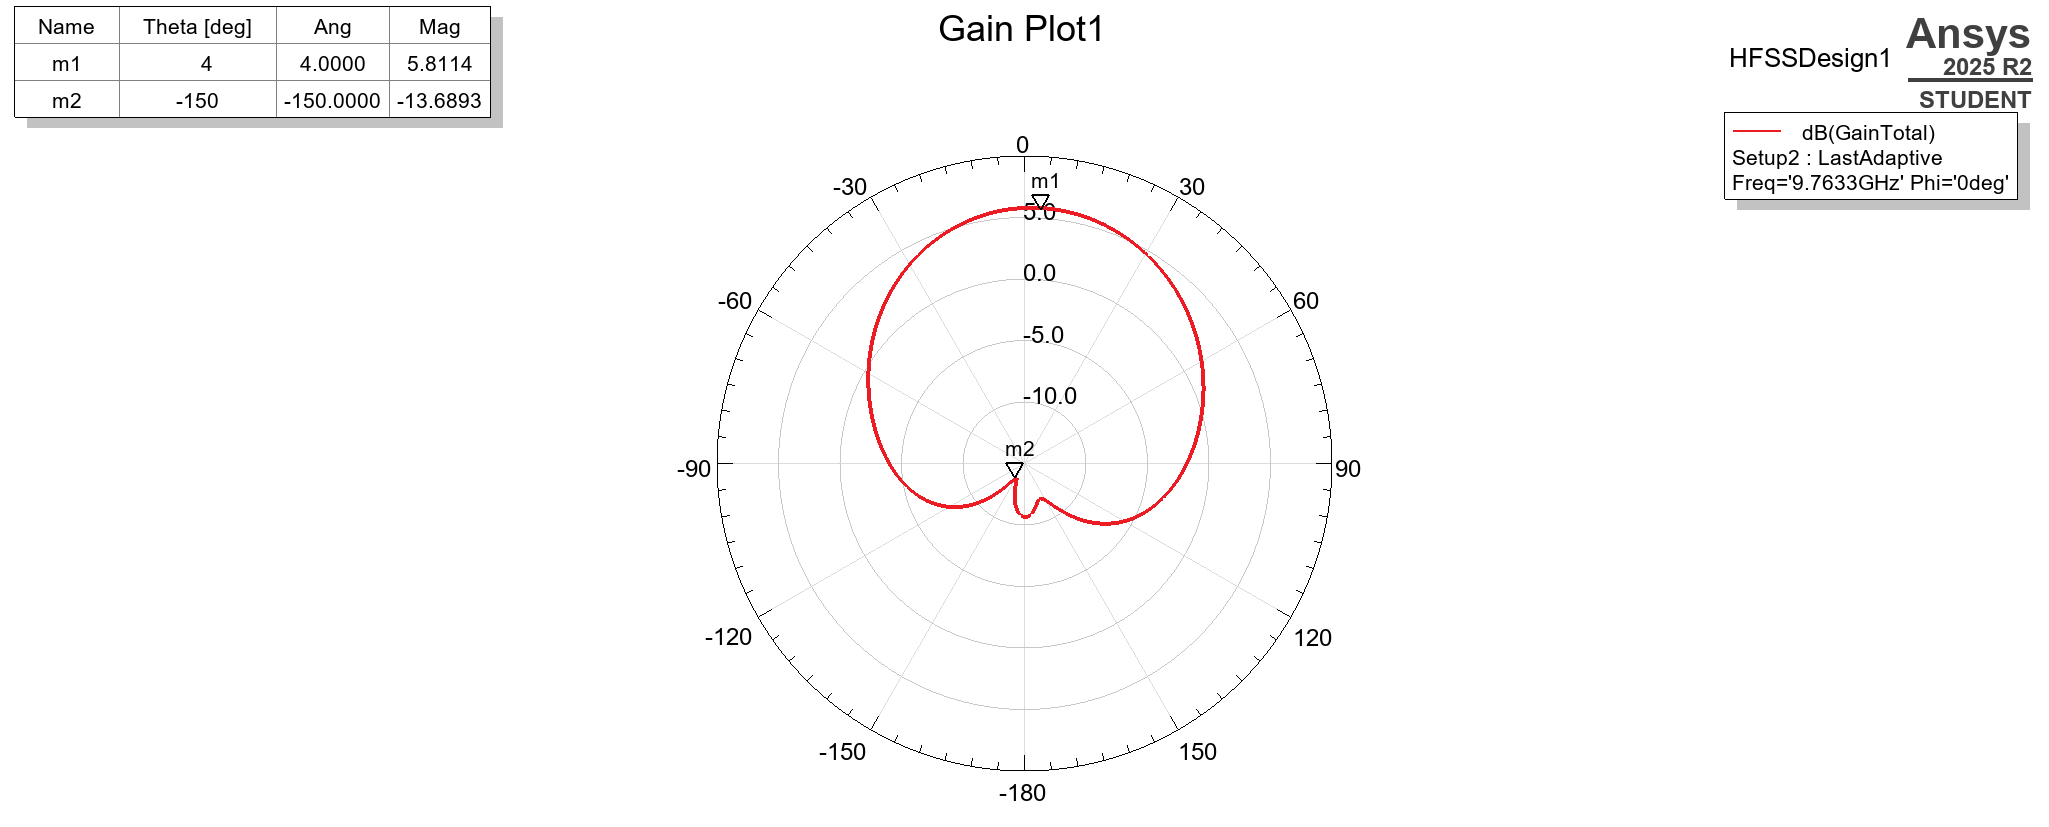
\includegraphics[width=1\textwidth]{p11.png}
    \caption{E 平面方向图}
    \label{fig:e_plane}
\end{figure}

【实验结果】：由仿真结果图 \ref{fig:e_plane}（E 平面方向图）可知：天线的 E 平面方向图呈方向性辐射，主瓣方向为 $\theta=4^\circ$，最大增益为 5.8114 dB。

\subsubsection{H 平面方向图}

\begin{enumerate}
    \item 右键单击工程树下的 \keyblue{Results} 节点，在弹出的菜单中选择 \keyblue{Create Far Fields Report}—\keyblue{Radiation Pattern} 命令，打开报告设置对话框。
    
    \item 在对话框左侧 \keyblue{Solution} 中选择 \keyblue{Setup2}，\keyblue{Geometry} 中选择 \keyblue{H Plane}，\keyblue{Primary Sweep} 中选择 \keyblue{Phi}，在 \keyblue{Category}、\keyblue{Quantity}、\keyblue{Function} 中依次选择 \keyblue{Gain}、\keyblue{GainTotal}、\keyblue{dB}，得到关于 H 平面的方向图如图 \ref{fig:h_plane} 所示。
\end{enumerate}

\begin{figure}[H]
    \centering
    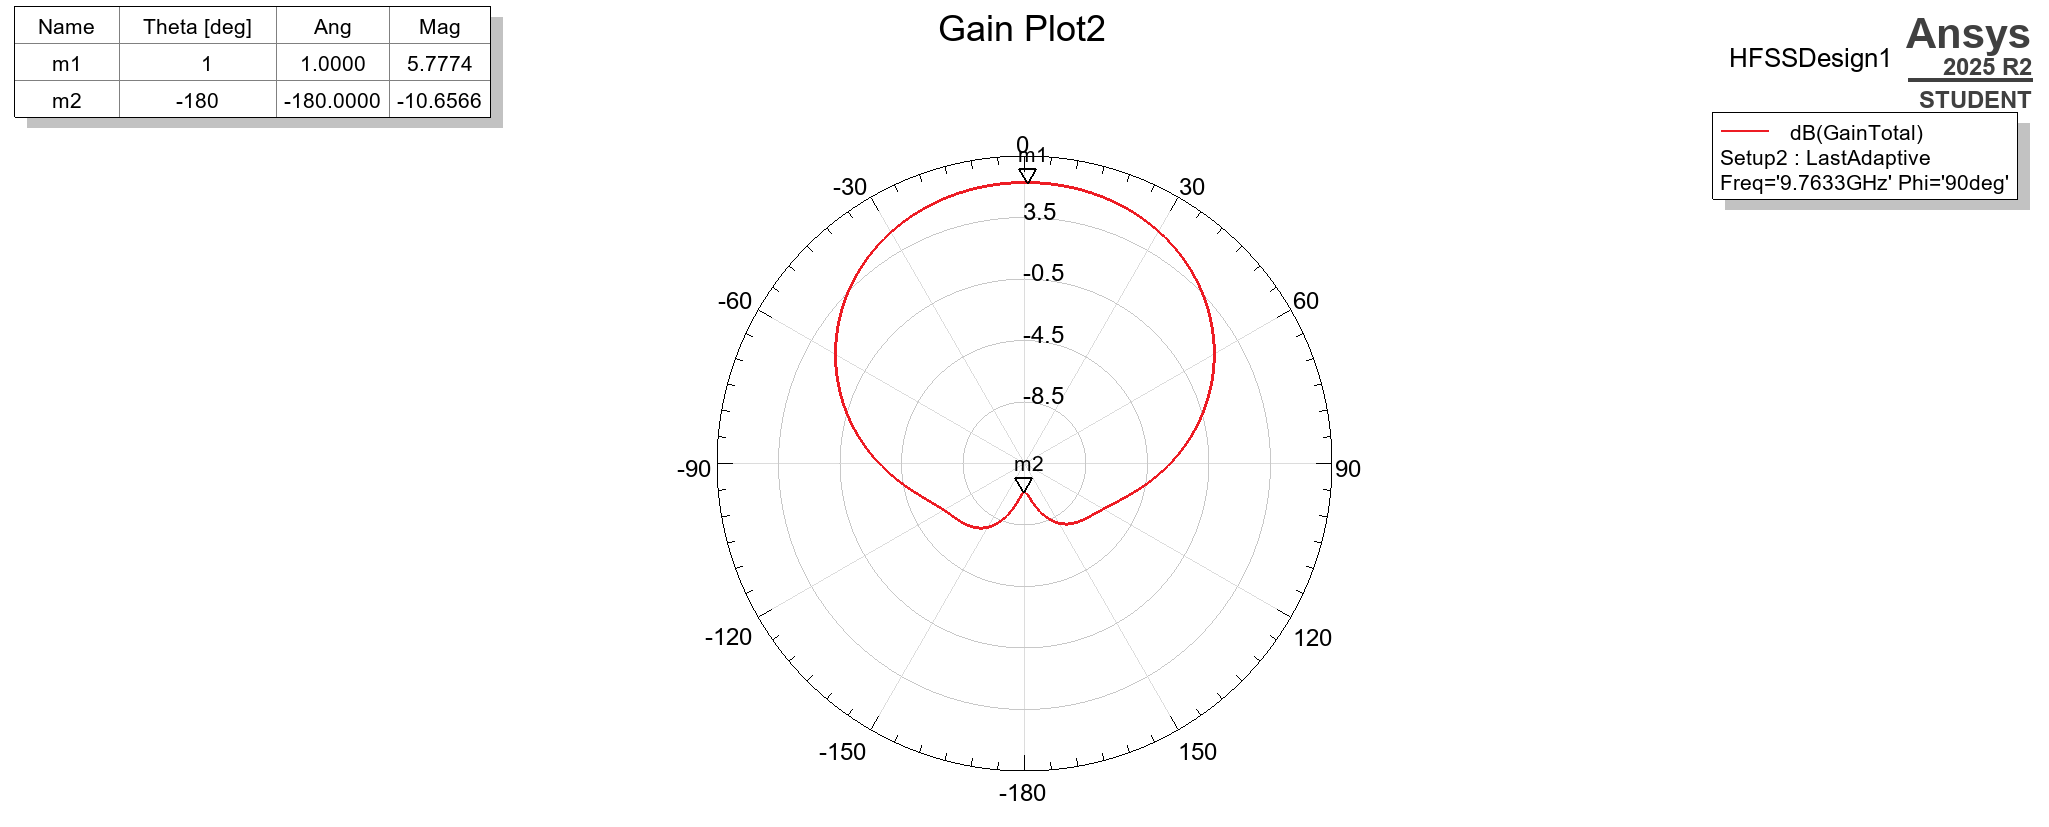
\includegraphics[width=1\textwidth]{p12_.png}
    \caption{H 平面方向图}
    \label{fig:h_plane}
\end{figure}

【实验结果】：由仿真结果图 \ref{fig:h_plane}（H 平面方向图）可知：天线的 H 平面方向图同样呈方向性辐射，主瓣方向为 $\theta=1^\circ$，最大增益为 5.7774 dB。

\subsubsection{三维方向图}

\begin{enumerate}
    \item 右键单击工程树下的 \keyblue{Results} 节点，在弹出的菜单中选择 \keyblue{Create Far Fields Report}—\keyblue{3D Polar Plot} 命令，打开报告设置对话框。
    
    \item 在对话框左侧 \keyblue{Solution} 中选择 \keyblue{Setup2: LastAdaptive}，\keyblue{Geometry} 中选择 \keyblue{3D Sphere}，在右侧 \keyblue{Primary Sweep} 中选择 \keyblue{Phi}，\keyblue{Secondary Sweep} 中选择 \keyblue{Theta}，下方 \keyblue{Category}、\keyblue{Quantity}、\keyblue{Function} 依次选择 \keyblue{Gain}、\keyblue{GainTotal}、\keyblue{dB}，点击 \keyblue{New Report}，再单击 \keyblue{Close}，得到天线的三维方向图如图 \ref{fig:3d_pattern} 所示。
\end{enumerate}

\begin{figure}[H]
    \centering
    \begin{minipage}[b]{0.5\linewidth}
        \centering
        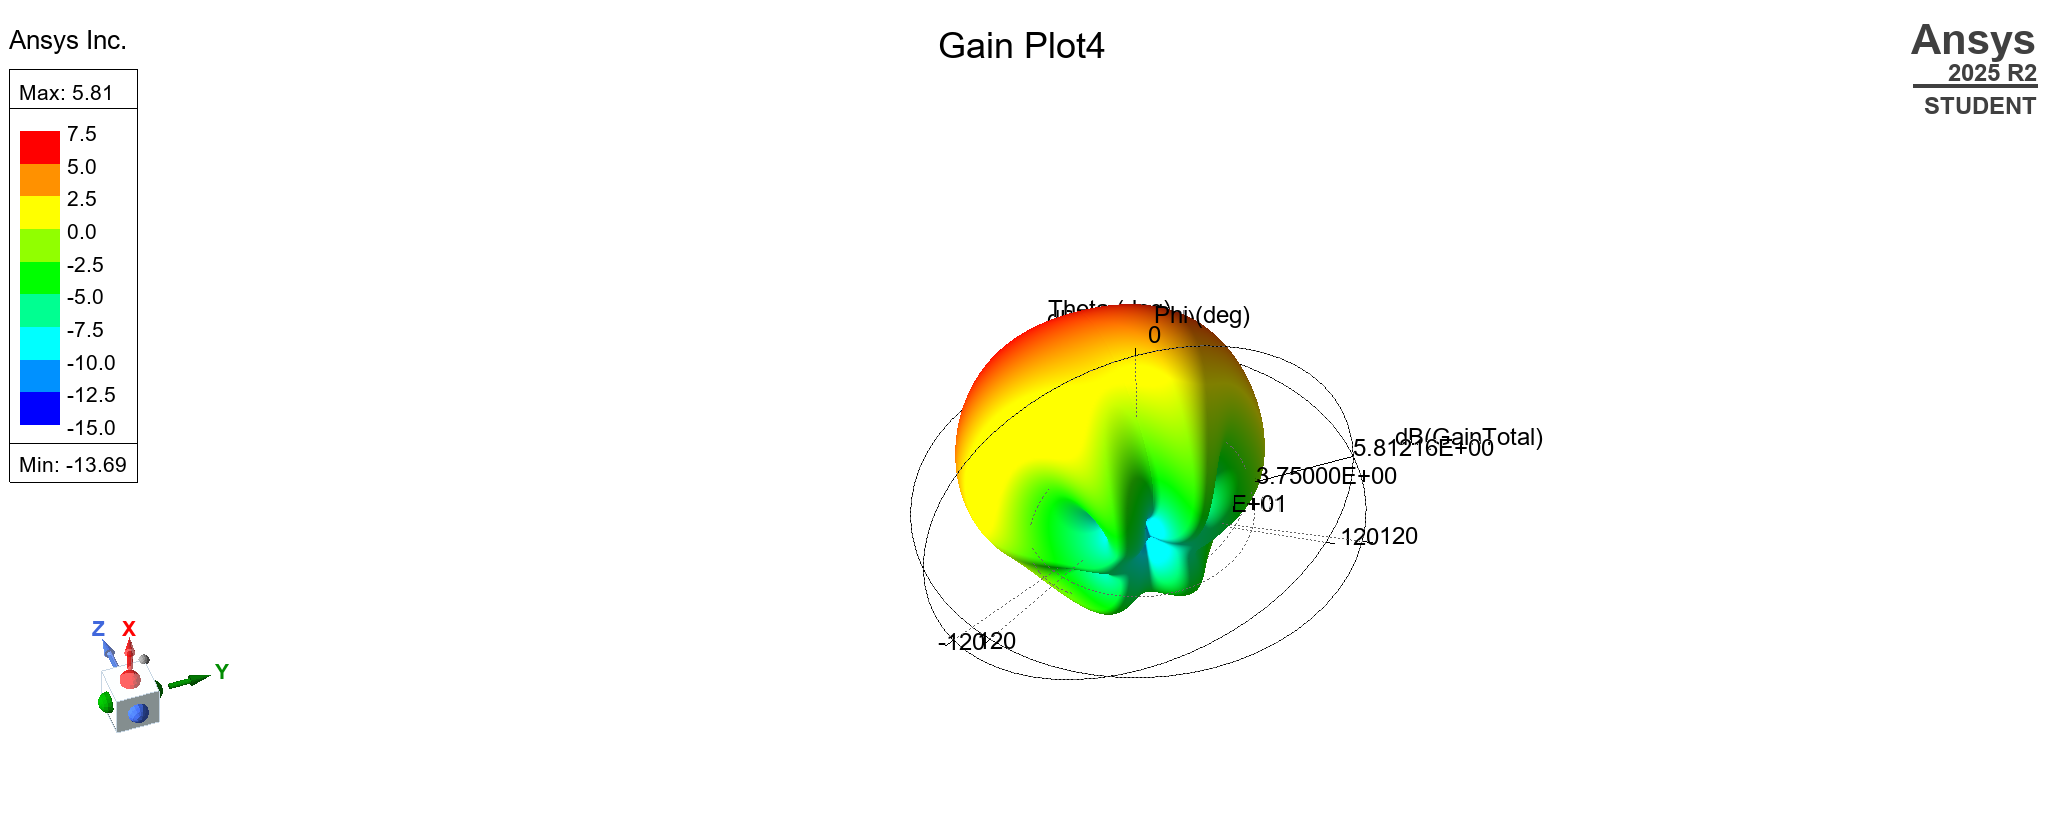
\includegraphics[width=0.9\textwidth]{p13_.png}
    \end{minipage}%
    \begin{minipage}[b]{0.5\linewidth}
        \centering
        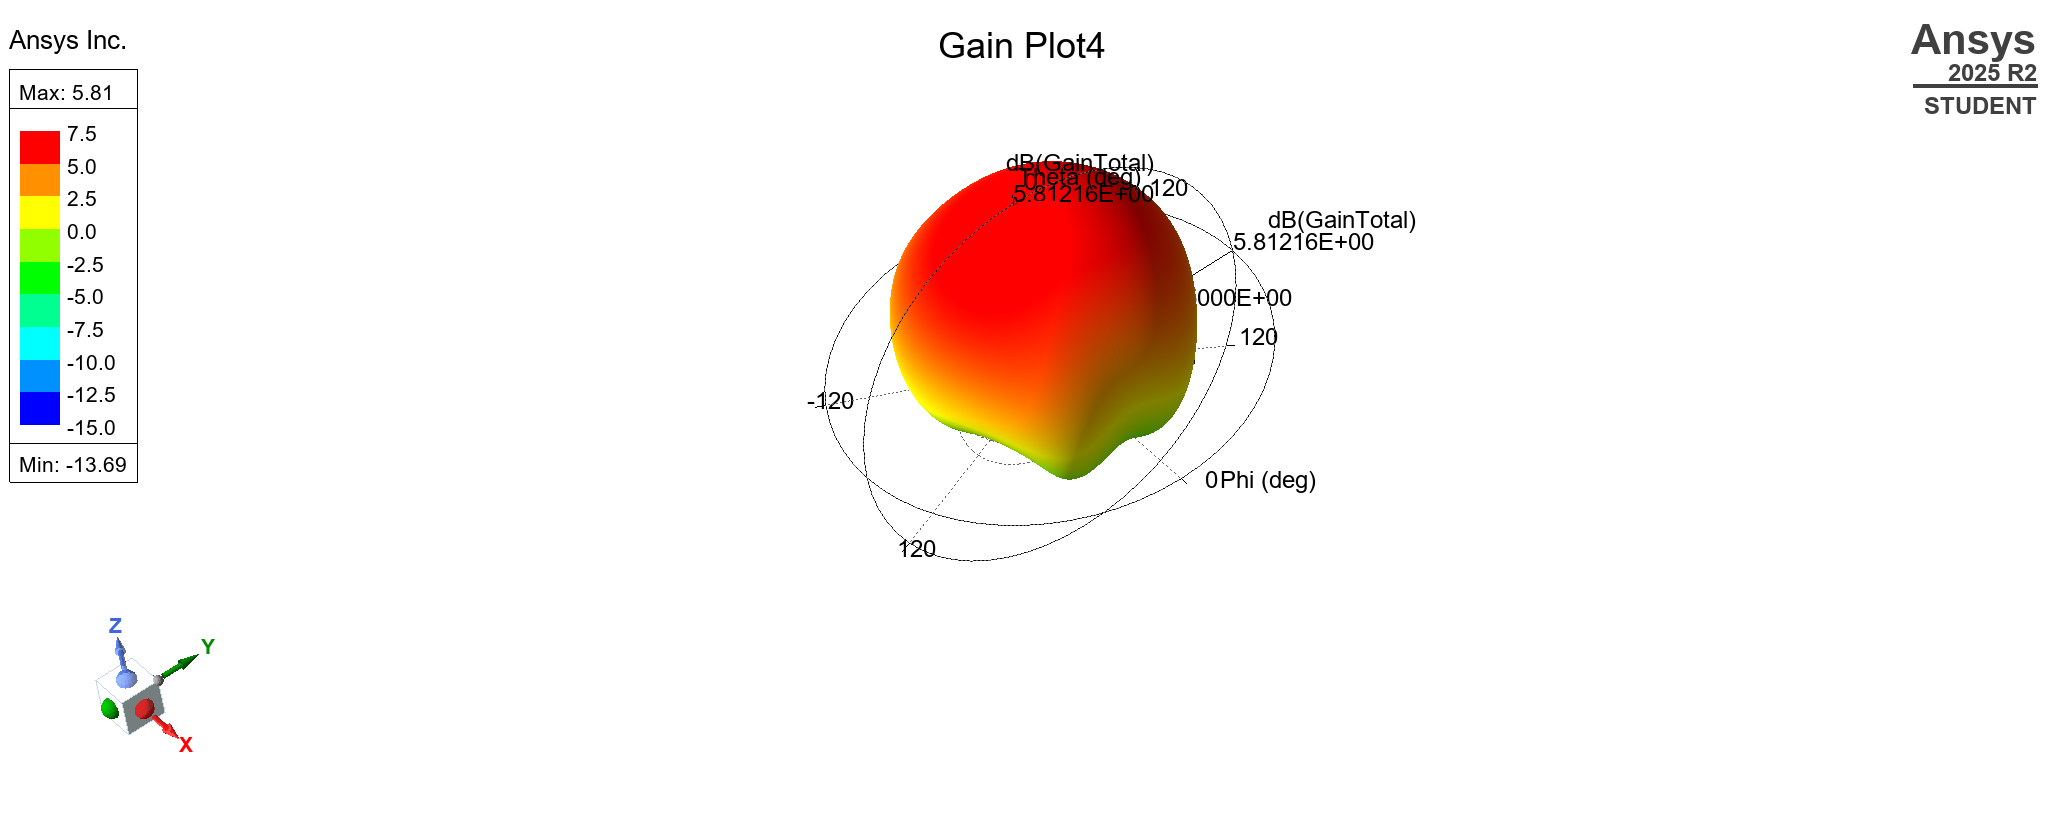
\includegraphics[width=0.9\textwidth]{p14_.png}
    \end{minipage}
    \caption{三维方向图}
    \label{fig:3d_pattern}
\end{figure}

【实验结果】：由仿真结果图 \ref{fig:3d_pattern}（三维方向图）可知：天线的三维方向图呈宽波束的定向辐射，能量主要集中在天线的法线方向（$\theta=0^\circ$）。
最大增益约为5.81dB，最小方向约为−13.69dB。

\section{实验结果分析}

\subsection{对比 HFSS 共振频率与理论10GHz的差异，并分析原因}

理论设计频率为 10 GHz，而 HFSS 仿真得到的实际谐振频率为 9.7633 GHz，仿真频率略低于理论频率，偏差约为 2.37\%。

\textbf{原因分析：}

\begin{enumerate}
    \item \textbf{经验公式误差：}理论计算中使用的有效介电常数 $\epsilon_{eff}$ 和边缘效应长度 $\Delta L$ 公式为近似经验公式，在厚基板和高介电常数情况下误差相对增大，与 HFSS 基于有限元法的精确全波电磁仿真存在固有偏差。
    
    \item \textbf{结构复杂性：}理论模型基于理想矩形贴片，未完全考虑馈线嵌入、切缝、四分之一波长阻抗变换器等结构带来的局部场扰动和附加电抗效应。
    
    \item \textbf{边界效应：}有限大地板与有限贴片边界引入附加电容效应，导致等效谐振频率下降。
    
    \item \textbf{数值误差：}HFSS 仿真中的网格剖分、自适应迭代次数、收敛容差等求解器设置也会带来一定的数值误差。
    
    \item \textbf{损耗与细节：}实际介质损耗、导体损耗以及几何细节（如圆角、倒角）未在理论解析模型中考虑。
\end{enumerate}

\subsection{在共振频率处给出E/H面辐射方向图与3D效能指标}

\textbf{E 平面方向图特性：}

如图 \ref{fig:e_plane} 所示，在谐振频率 9.7633 GHz 处，E 平面方向图呈现余弦分布近似的主瓣，副瓣电平较低，主瓣方向为 $\theta$近似于$0^\circ$，辐射特性良好。

\textbf{H 平面方向图特性：}

如图 \ref{fig:h_plane} 所示，H 平面主瓣相对 E 平面更宽，零点位置与贴片等效缝隙模型理论预测一致，波束宽度大于 E 平面。

\textbf{3D 效能指标：}

如图 \ref{fig:3d_pattern} 所示，三维方向图呈宽波束定向辐射，能量主要集中在天线法线方向（$\theta=0^\circ$）。天线在主辐射方向的最大增益为 5.81 dB，与典型单贴片微带天线的性能水平（约 5-6 dB）一致，表明天线设计合理有效。

\section{实验探究}

\subsection{d0参数扫参}

为在10GHz 处获得更佳的匹配与辐射性能，进行了以贴片几何尺寸为主的参数优
化。如2.5切缝宽度d0计算中所说，此时的d0不一定为最优解，故取d0在 $0.0193 cm \sim 0.0483 cm$
中取Step Size为0.001 cm进行扫参。

\begin{figure}[H]
    \centering
    \begin{minipage}[b]{0.5\linewidth}
        \centering
        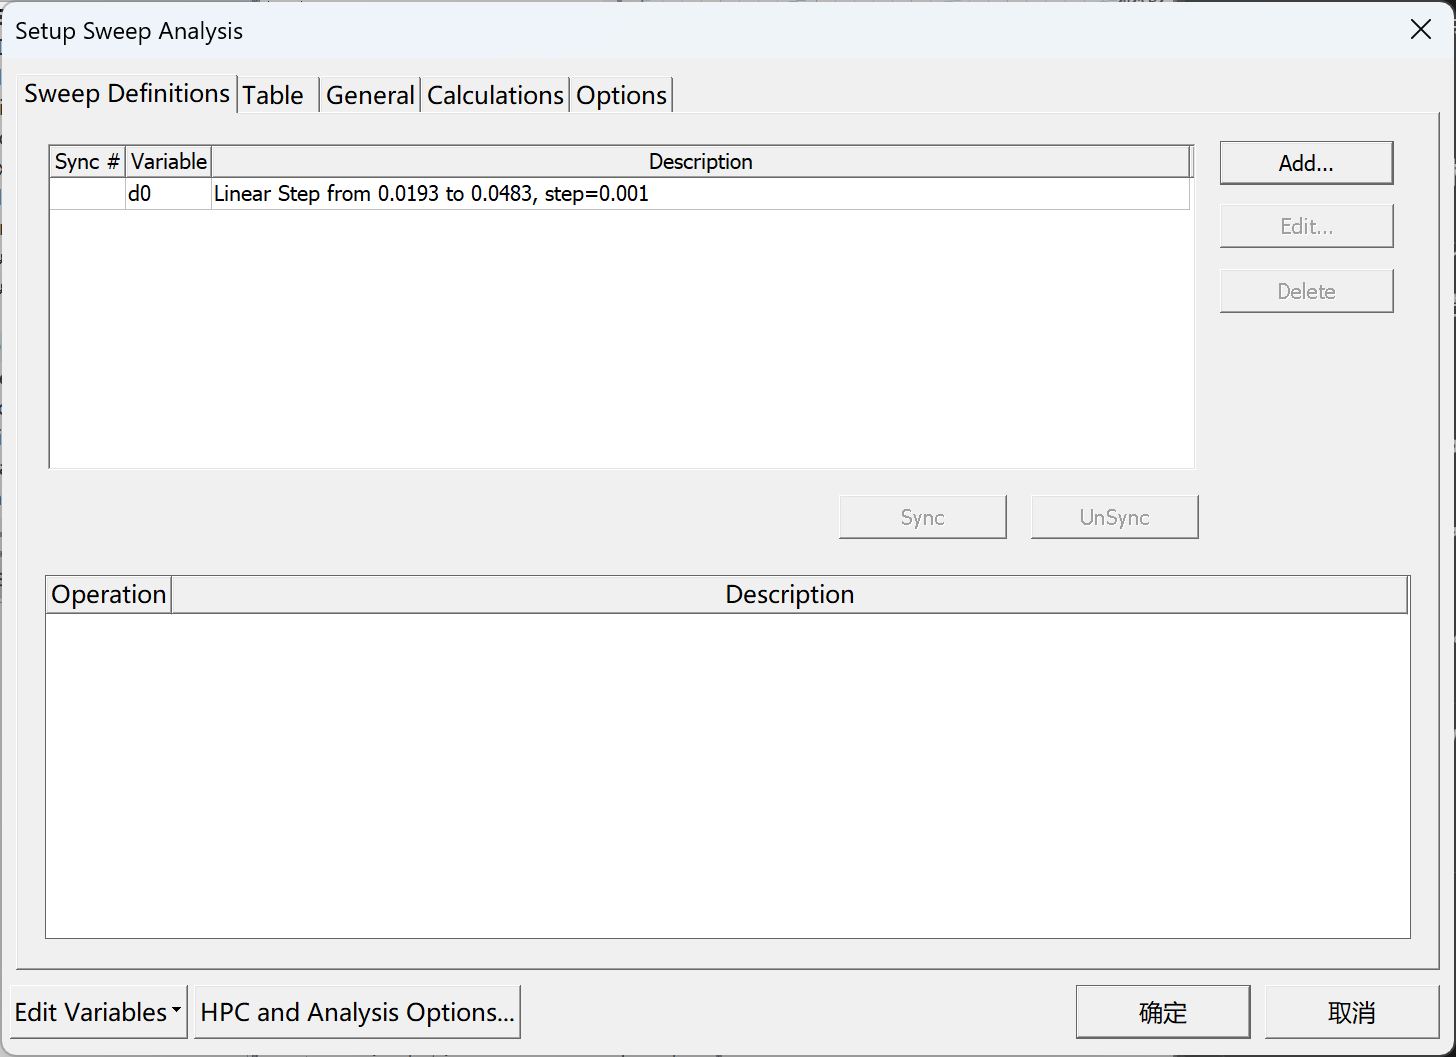
\includegraphics[width=0.9\textwidth]{p15.png}
    \end{minipage}%
    \begin{minipage}[b]{0.5\linewidth}
        \centering
        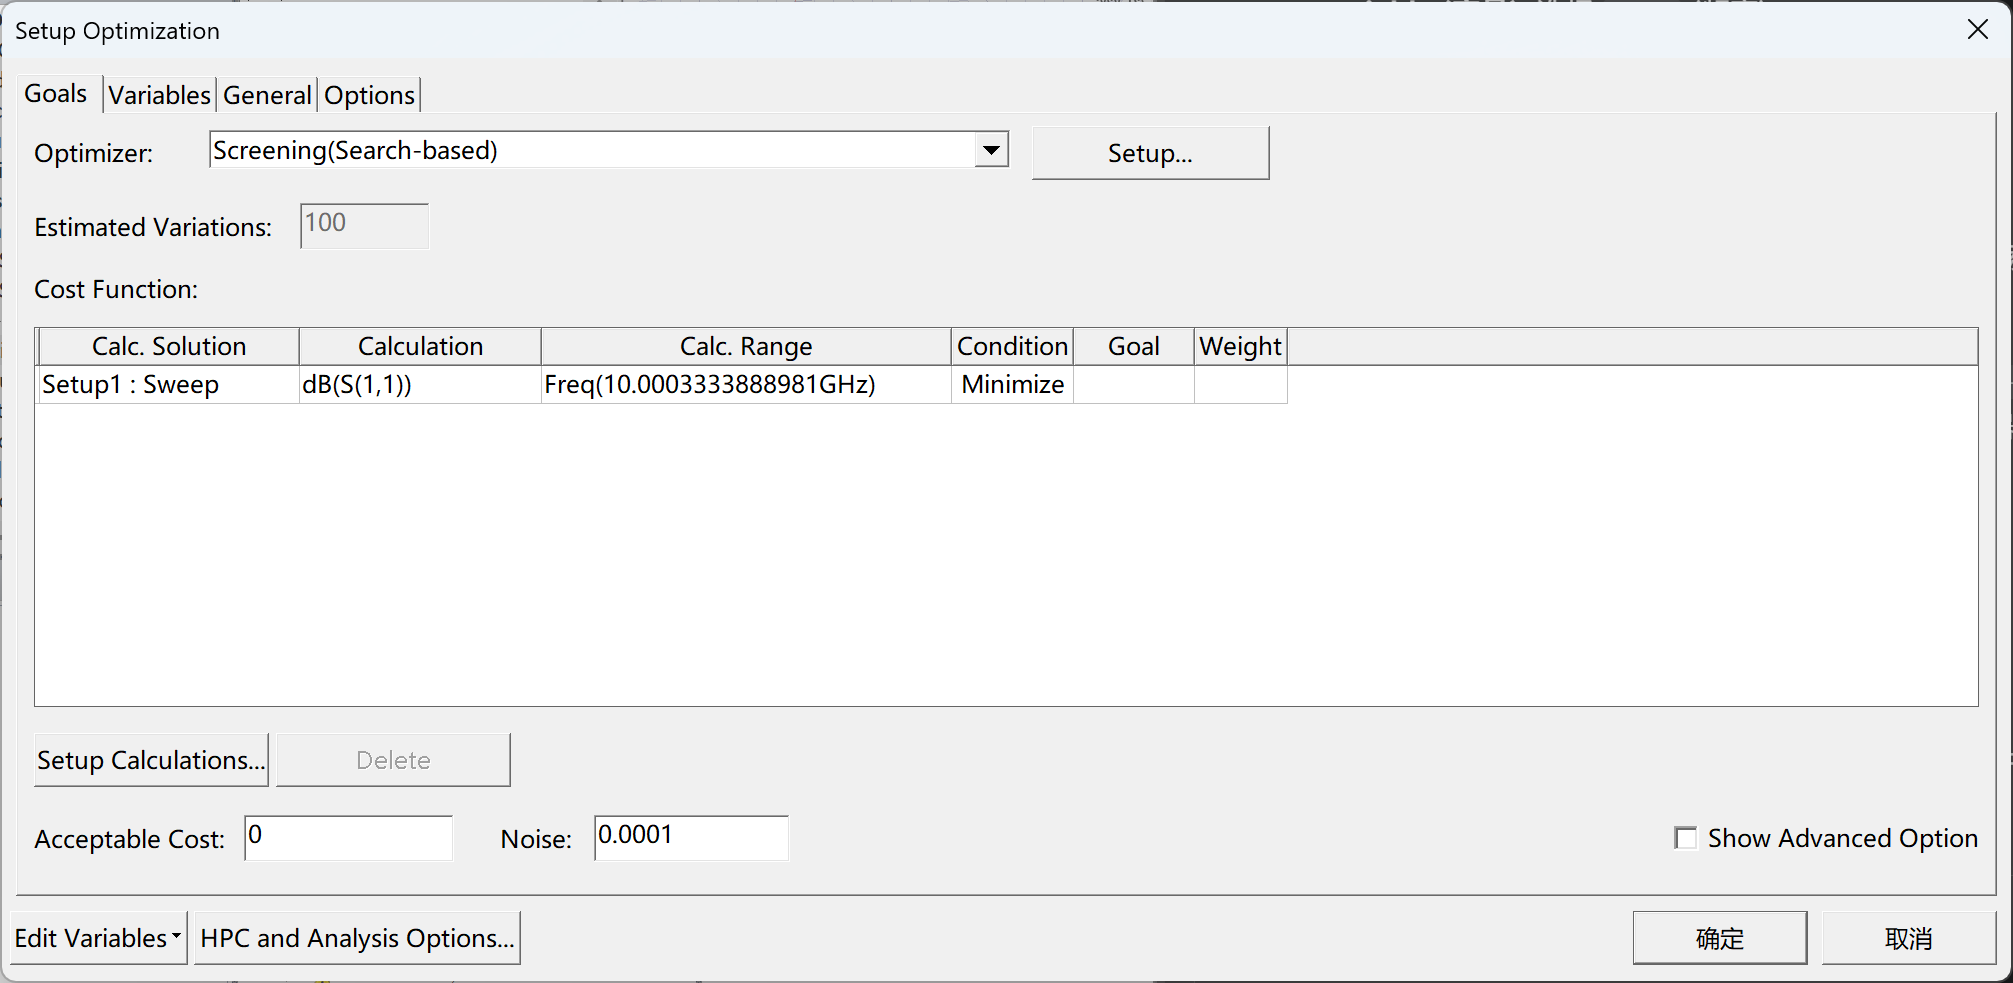
\includegraphics[width=0.9\textwidth]{p16.png}
    \end{minipage}
    \caption{d0参数扫参设置}
    \label{fig:d0_sweep}
\end{figure}

\begin{figure}[H]
    \centering
    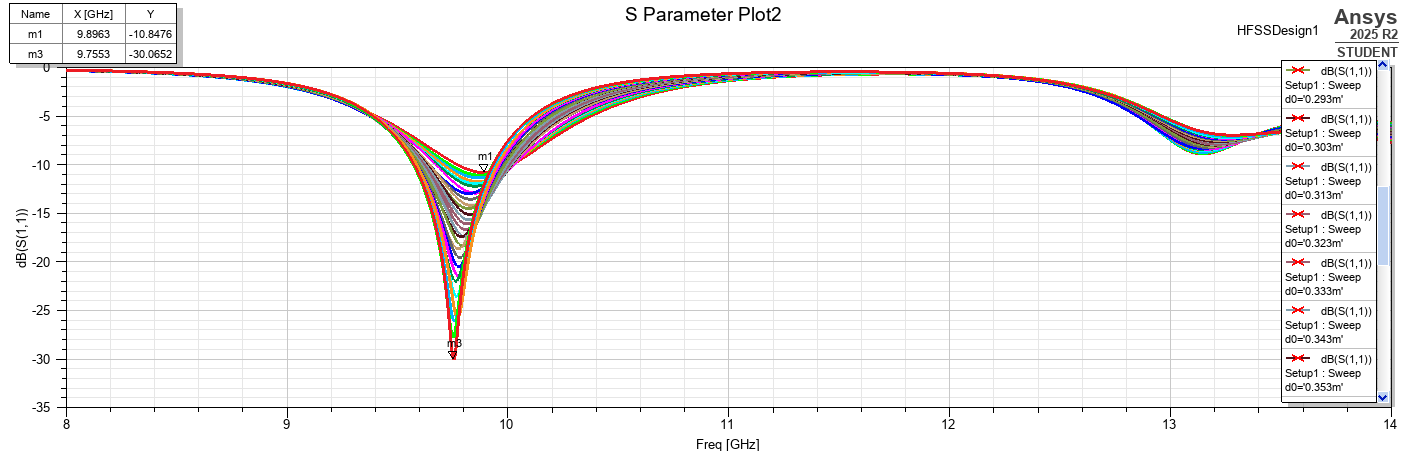
\includegraphics[width=1\textwidth]{p20.png}
    \caption{d0参数等距扫参结果}
    \label{fig:d0_result1}
\end{figure}

采取另一种方法进行扫参，即让d0在 $0.0193 cm \sim 0.0483 cm$ 中扫参，目标函数优先最小化|S11(10GHz)|，让HFSS自行迭代，结果如Figure \ref{fig:d0_result2}所示。

\begin{figure}[H]
    \centering
    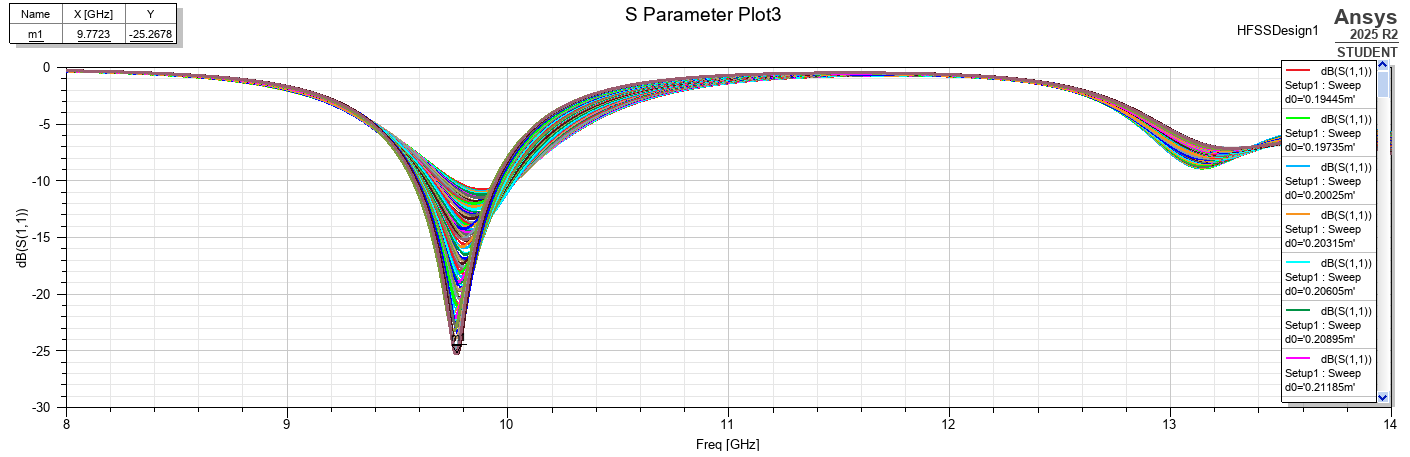
\includegraphics[width=1\textwidth]{p19.png}
    \caption{d0参数自优化扫参结果}
    \label{fig:d0_result2}
\end{figure}

【实验结果】：两个扫参结果均说明，随着d0参数的减小，虽然谐振频率有所上移，但回波损耗显著上升，甚至接近-10dB，
说明较难通过d0参数来让天线良好的工作在10GHz，要采取别的方式，下面通过W/L扫参来调整谐振频率。

\subsection{W/L扫参}

接下来试图更改W与L的值，以在10GHz处获得更佳的匹配与辐射性能，如下图进行W/L参数扫参设置：

\begin{figure}[H]
    \centering
    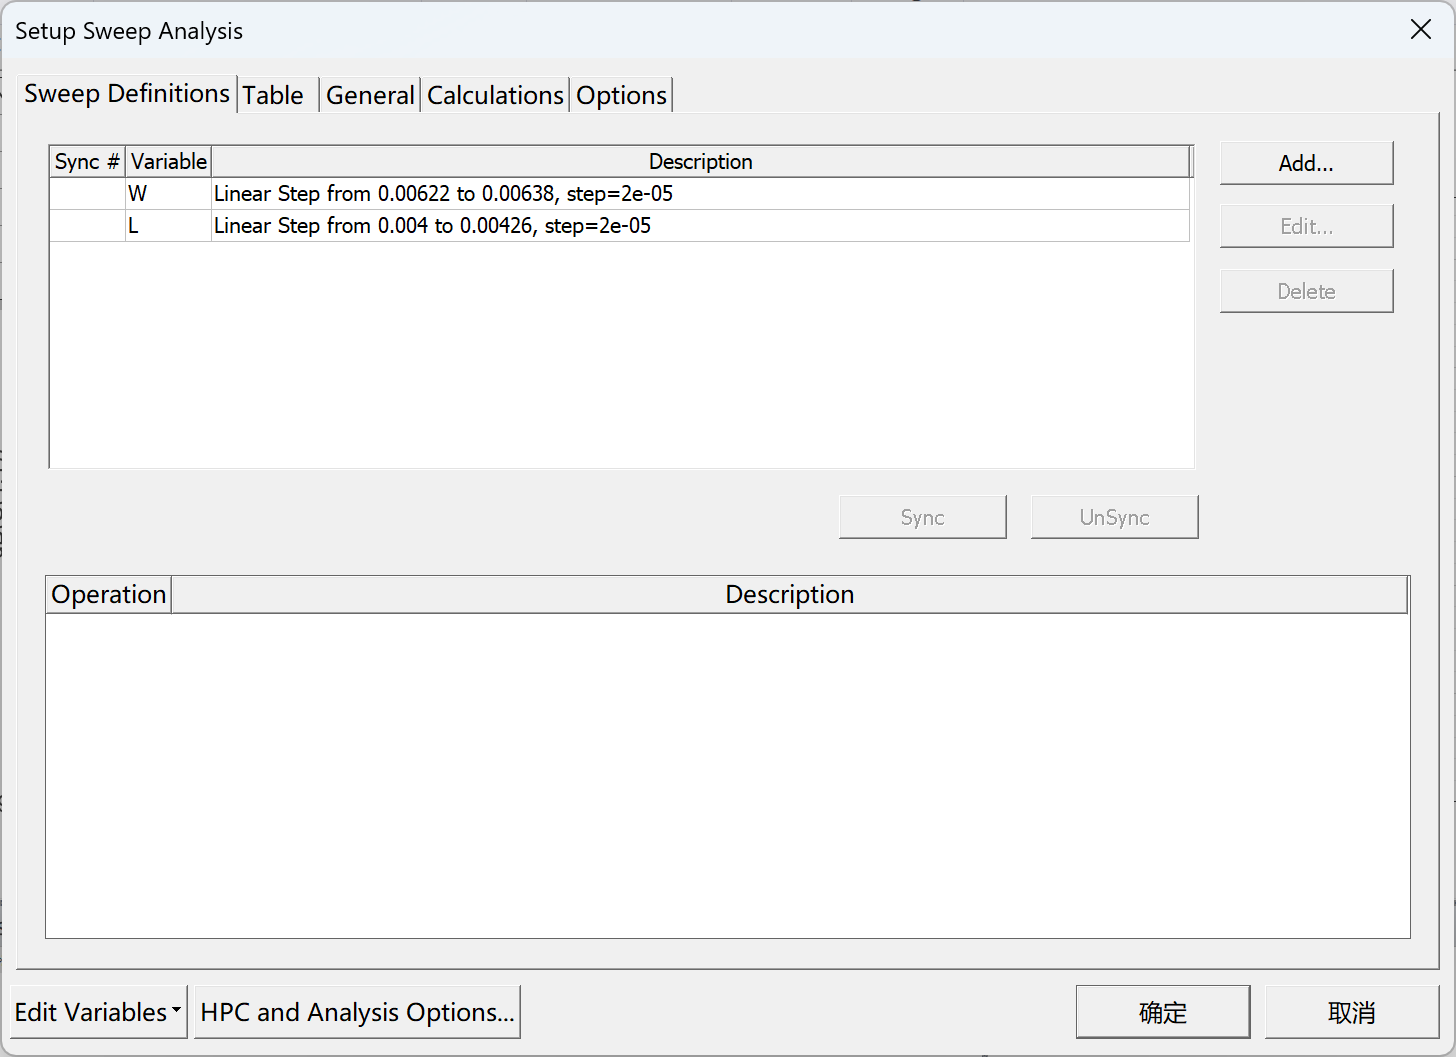
\includegraphics[width=0.9\textwidth]{p25.png}
    \caption{W/L参数扫参设置}
\end{figure}

W/L参数扫描结果如下图所示:

\begin{figure}[H]
    \centering
    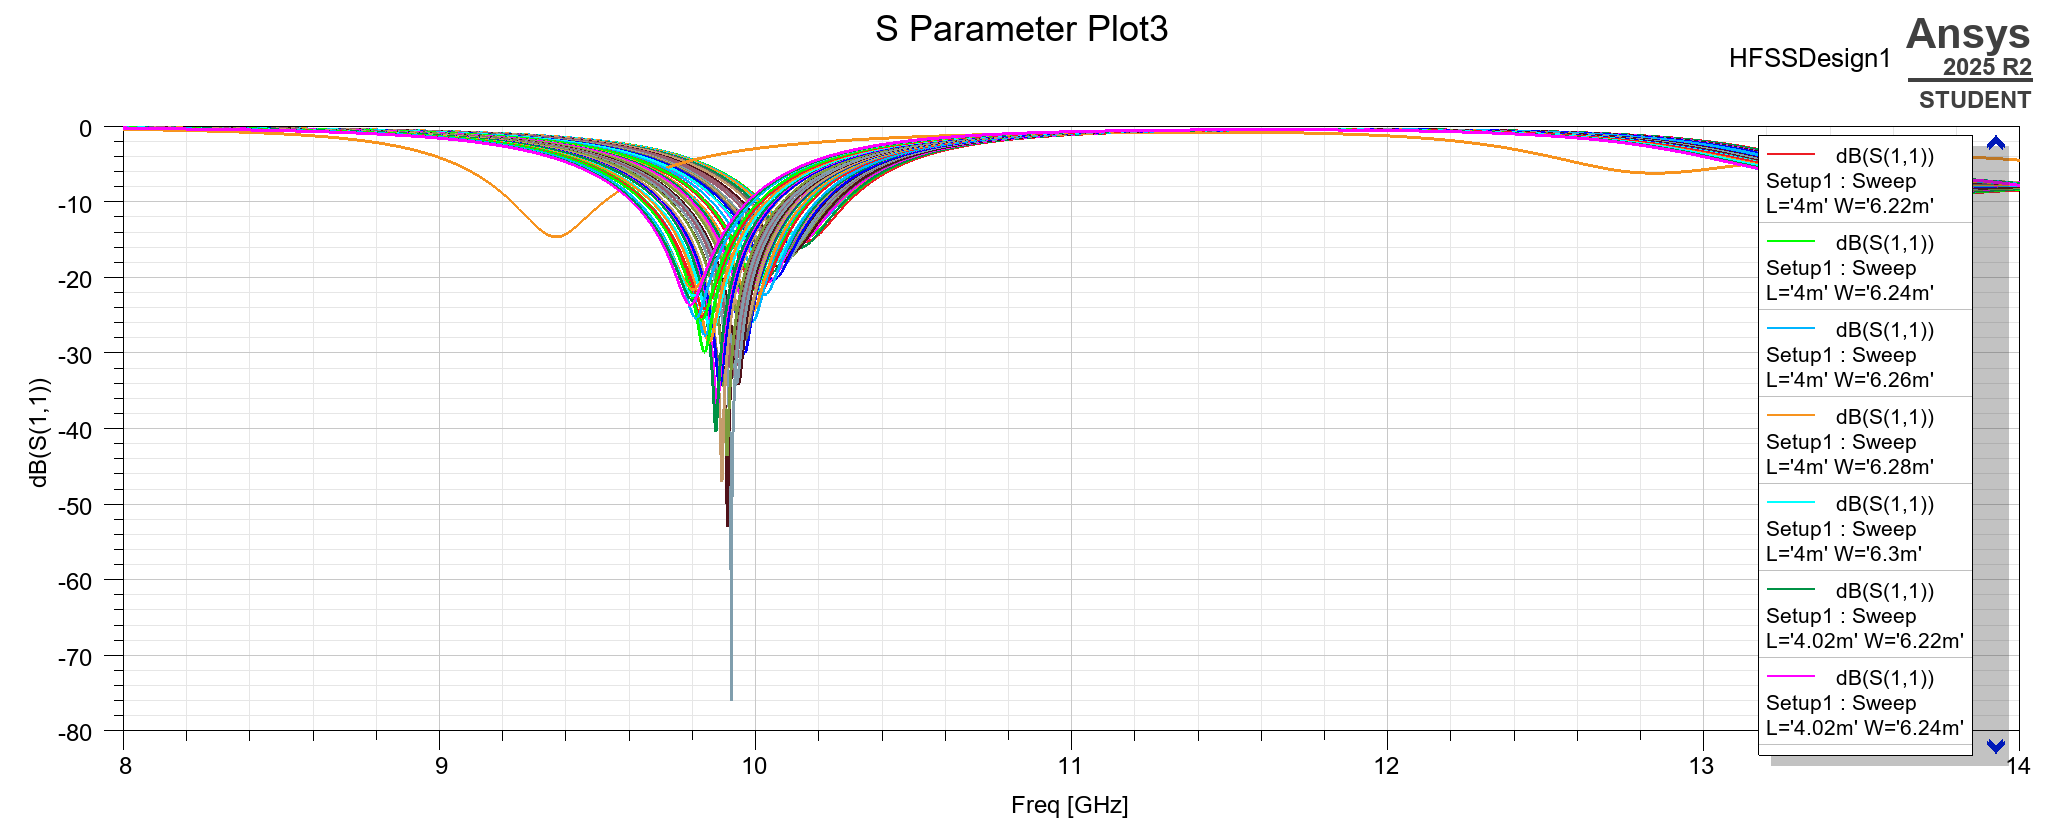
\includegraphics[width=1\textwidth]{p21.png}
    \caption{W/L参数扫参结果}
\end{figure}

\begin{figure}[H]
    \centering
    \begin{minipage}[b]{0.45\linewidth}
        \centering
        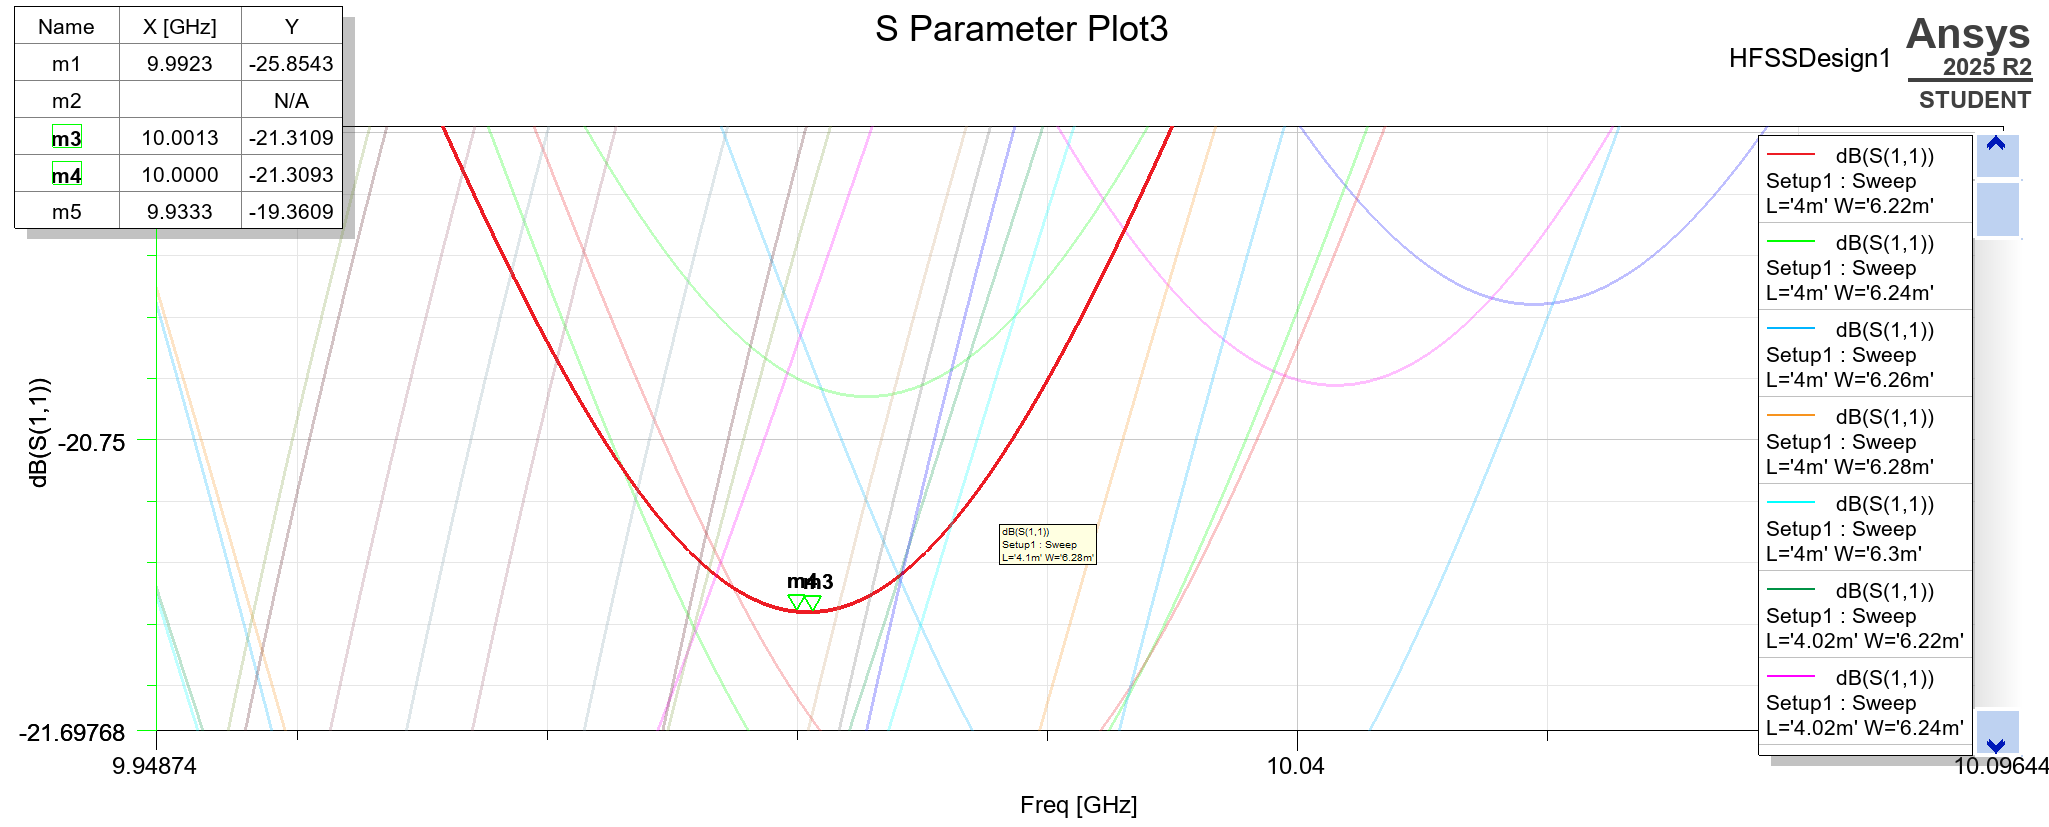
\includegraphics[width=0.9\textwidth]{p23.png}
        \caption{W=0.628cm,L=0.41cm}
            
    \end{minipage}%
    \begin{minipage}[b]{0.45\linewidth}
        \centering
        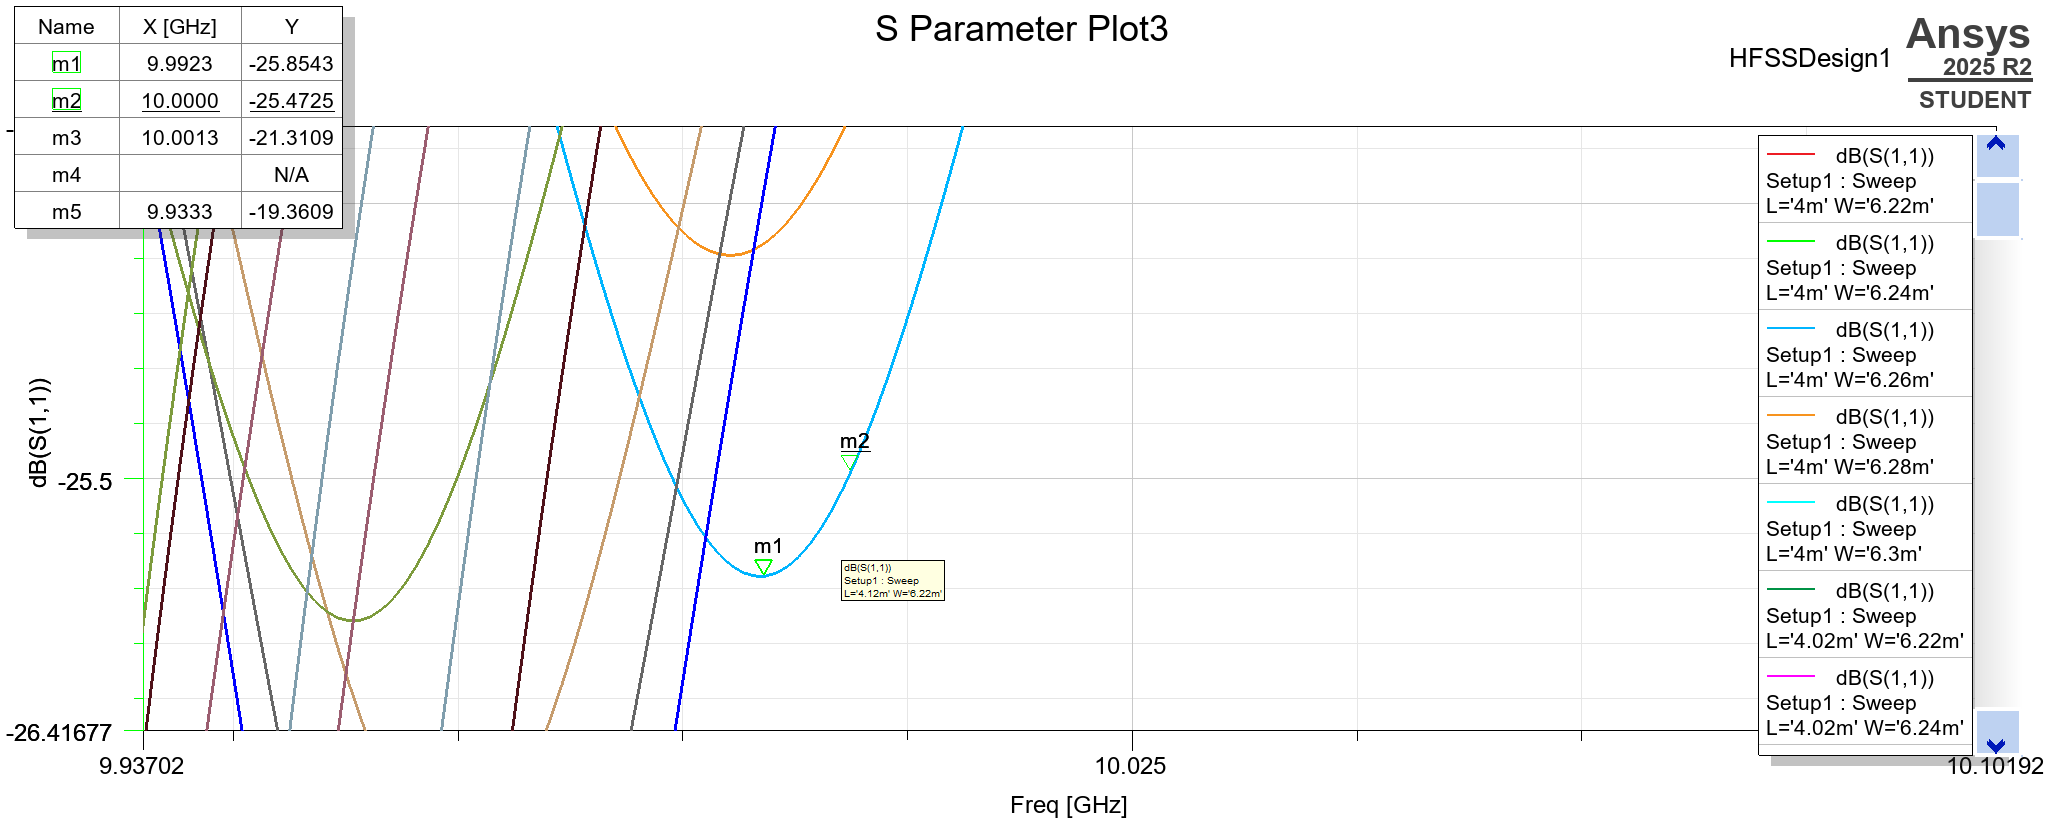
\includegraphics[width=0.9\textwidth]{p24.png}
        \caption{W=0.622cm,L=0.412cm}

    \end{minipage}
\end{figure}



由仿真图中可以看出，

在$ W=0.628cm,L=0.41cm$时，谐振频率为10.0013GHz，10GHz下的回波损耗为-21.3093dB，此时谐振频率与10GHz最接近。

在$ W=0.622cm,L=0.412cm$时，谐振频率为9.9923GHz，10GHz下的回波损耗为-25.4725dB，此时10GHz下的回波损耗最小。

\subsection{W/L优化仿真}

采取优化后的W与L值进行仿真,此处为了使10GHz处的回波损耗更小，取$ W=0.622cm,L=0.412cm$进行仿真，结果如下:

\subsubsection{回波损耗}

\begin{figure}[H]
    \centering
    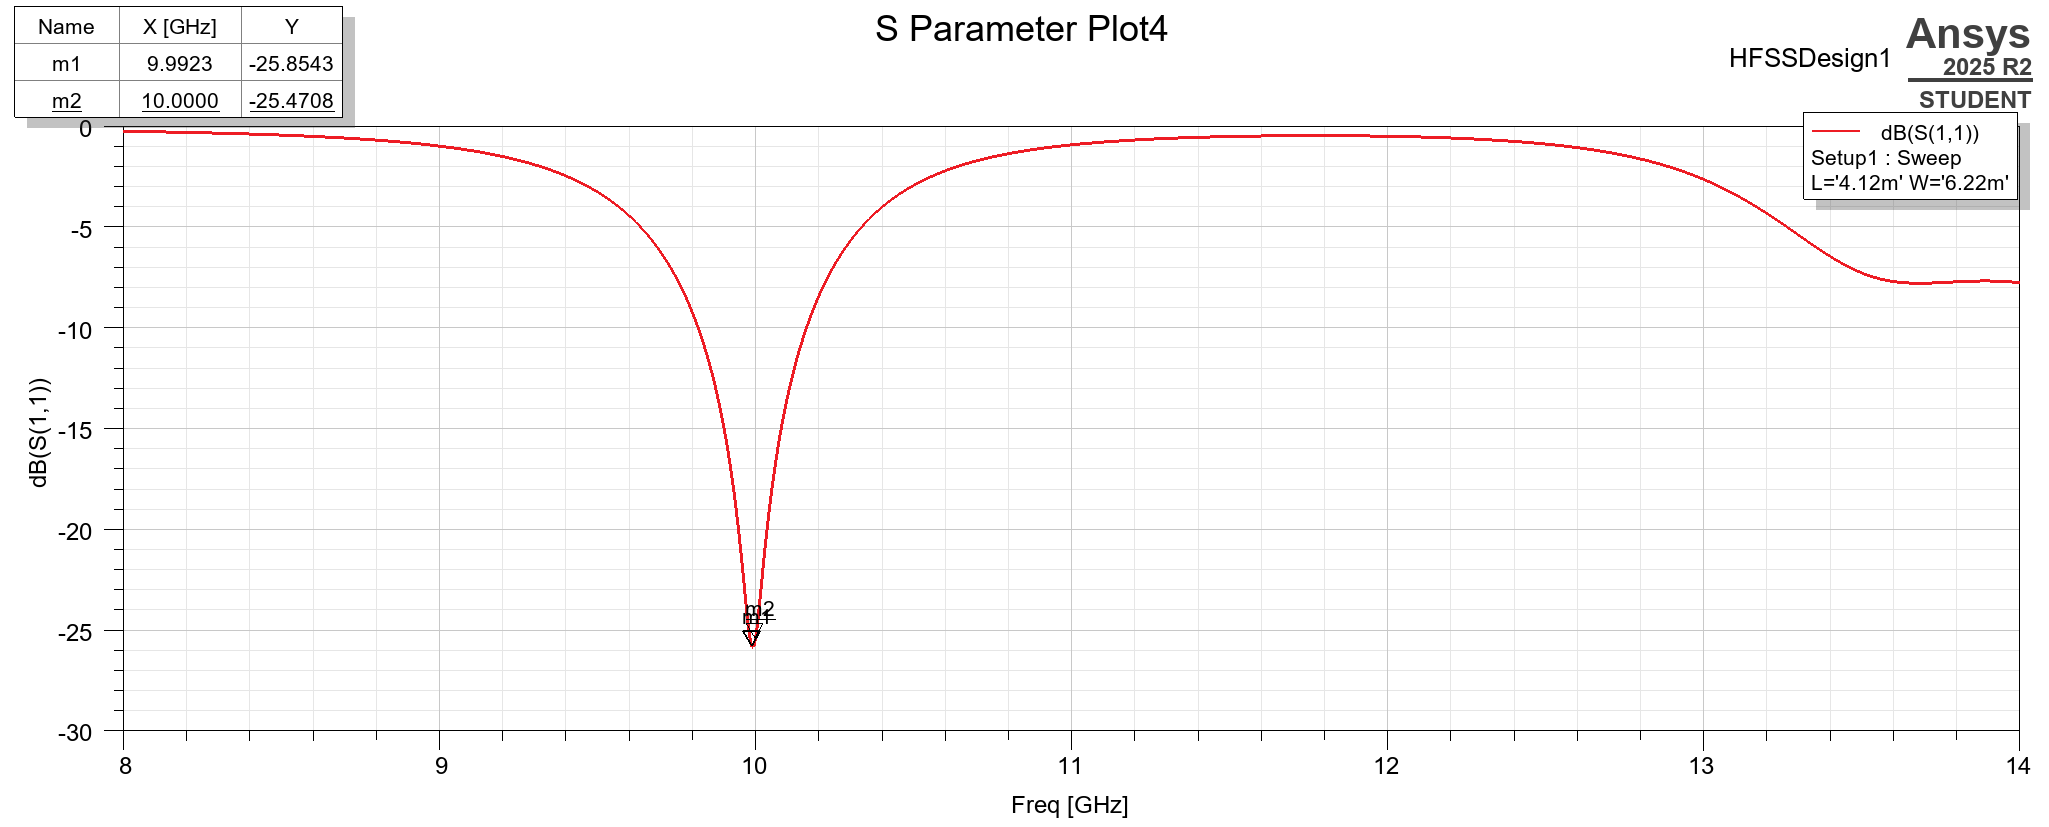
\includegraphics[width=1\textwidth]{p26.png}
    \caption{回波损耗}
\end{figure}

【实验结论】：经过 W/L 参数优化（$W=0.622$ cm, $L=0.412$ cm），天线在目标频率 10.00 GHz 处的回波损耗达到了 -25.4708 dB，同时实际谐振点位于 9.9923 GHz（$S_{11} = -25.8543$ dB）。这表明优化后的尺寸成功地将谐振频率修正到了非常接近 10 GHz 的位置，并实现了优异的阻抗匹配。

\subsubsection{输入阻抗}

\begin{figure}[H]
    \centering
    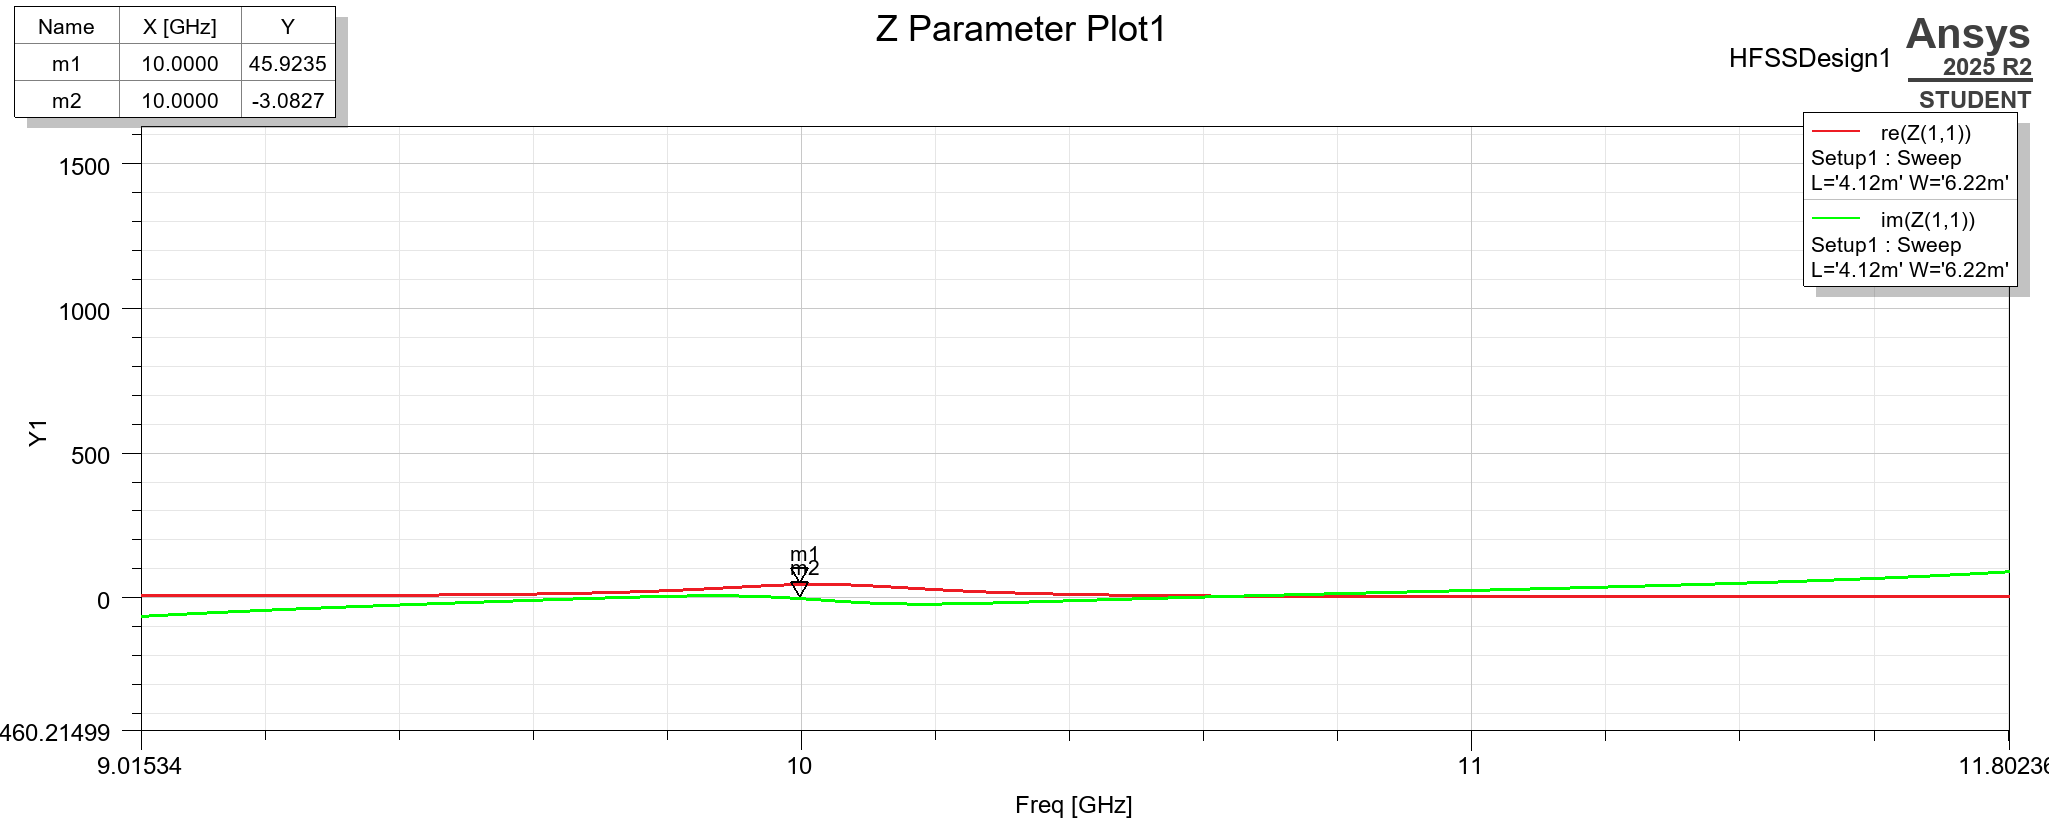
\includegraphics[width=1\textwidth]{p28.png}
    \caption{输入阻抗}
\end{figure}

【实验结论】：在 10.00 GHz 频率下，优化后天线在端口处的输入阻抗实部为 45.9235 $\Omega$，虚部为 -3.0827 $\Omega$。该阻抗值非常接近 50 $\Omega$ 的系统特性阻抗，且电抗（虚部）很小，这进一步验证了 6.3.1 中观察到的良好回波损耗是由优异的阻抗匹配所实现的。

\subsubsection{方向图}


\begin{figure}[H]
    \centering
    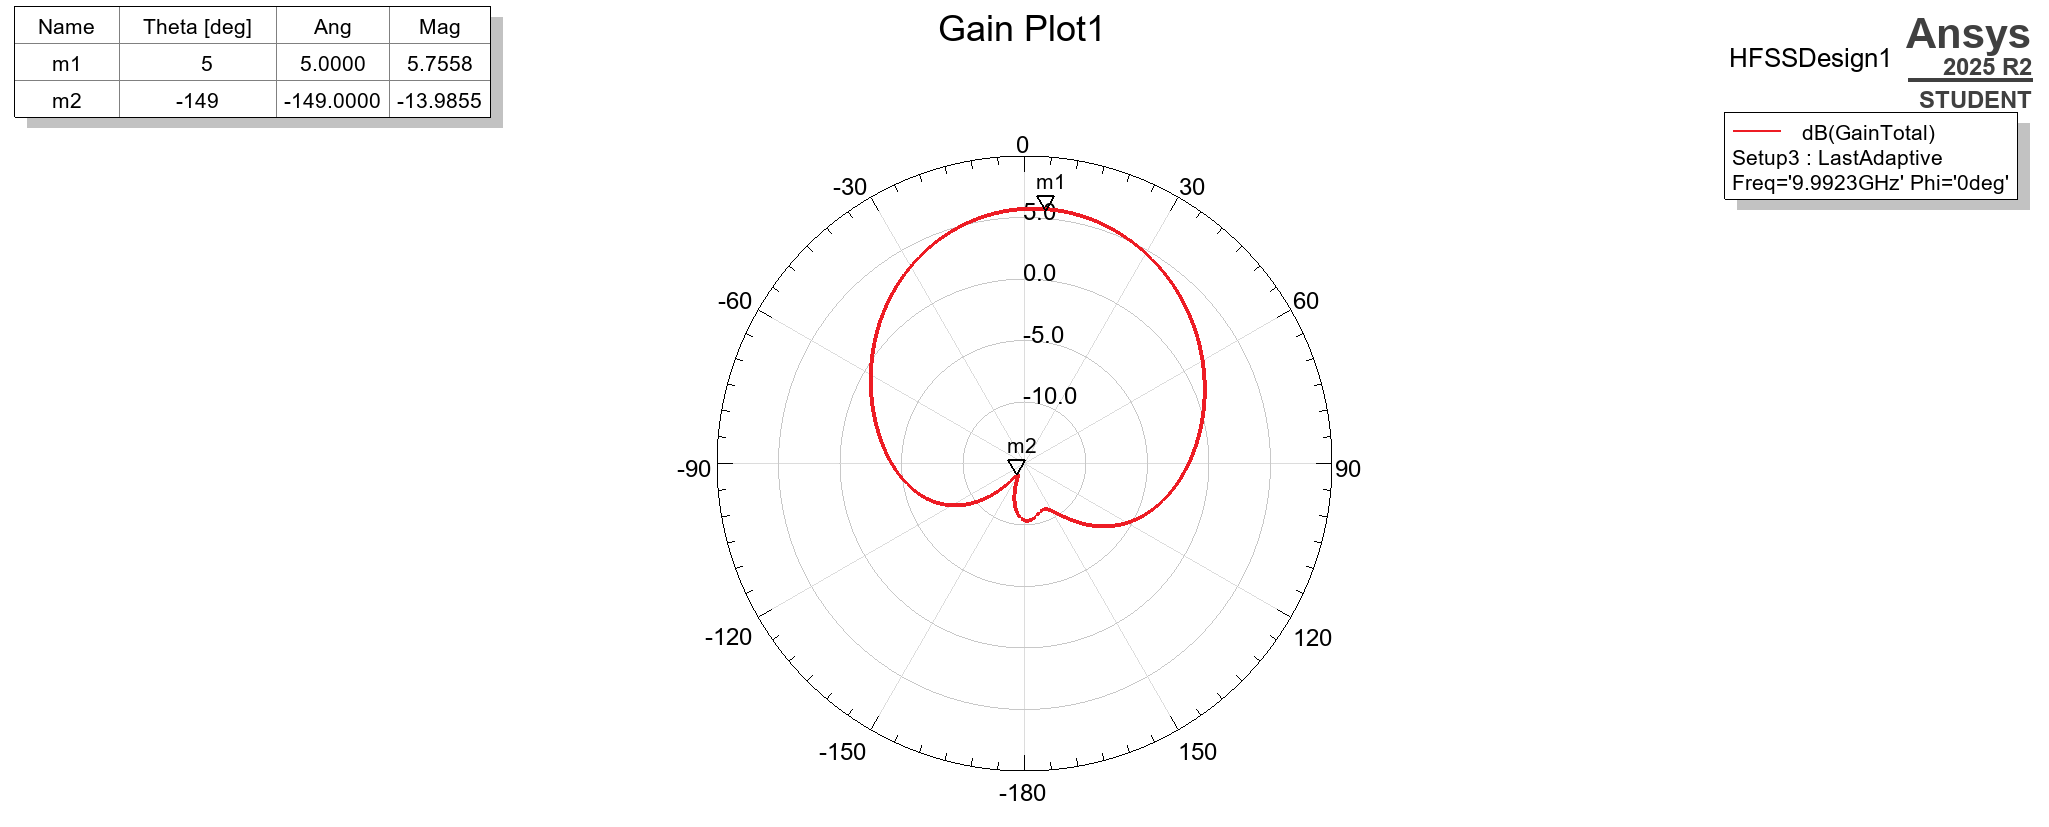
\includegraphics[width=1\textwidth]{p29.png}
    \caption{E平面方向图}
\end{figure}


\begin{figure}[H]
    \centering
    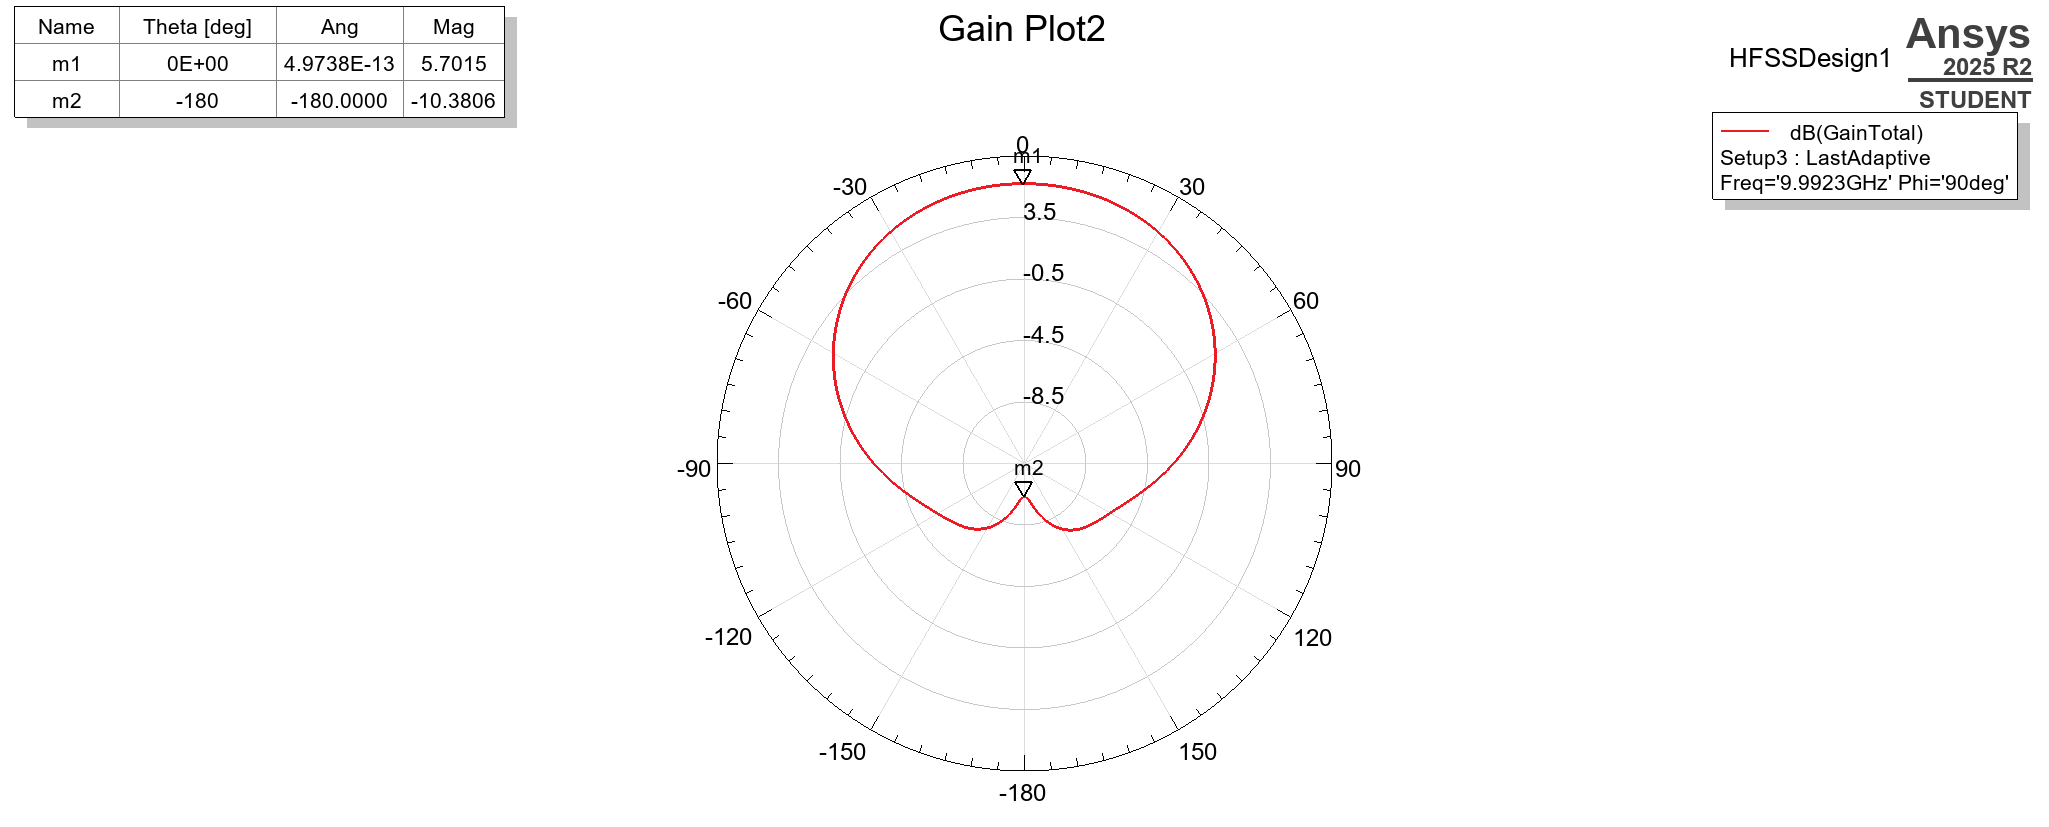
\includegraphics[width=1\textwidth]{p30.png}
    \caption{H平面方向图}
\end{figure}


\begin{figure}[H]
    \centering
    \begin{minipage}[b]{0.5\linewidth}
        \centering
        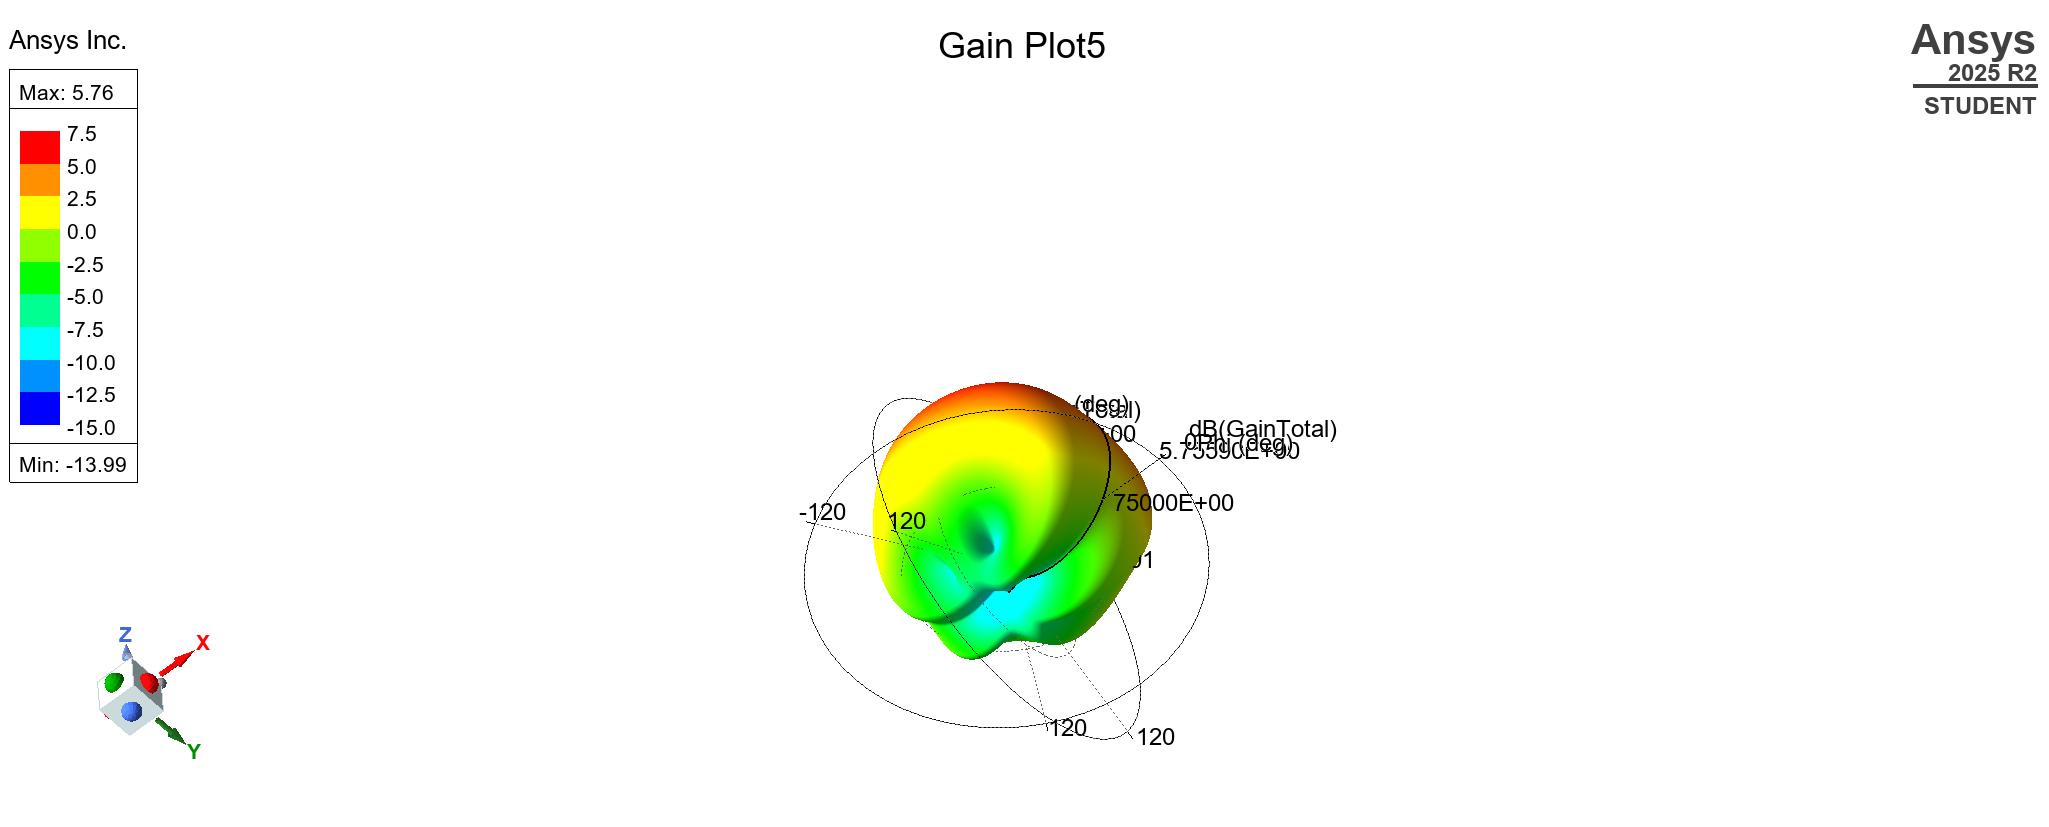
\includegraphics[width=0.9\textwidth]{p31.png}
    \end{minipage}%
    \begin{minipage}[b]{0.5\linewidth}
        \centering
        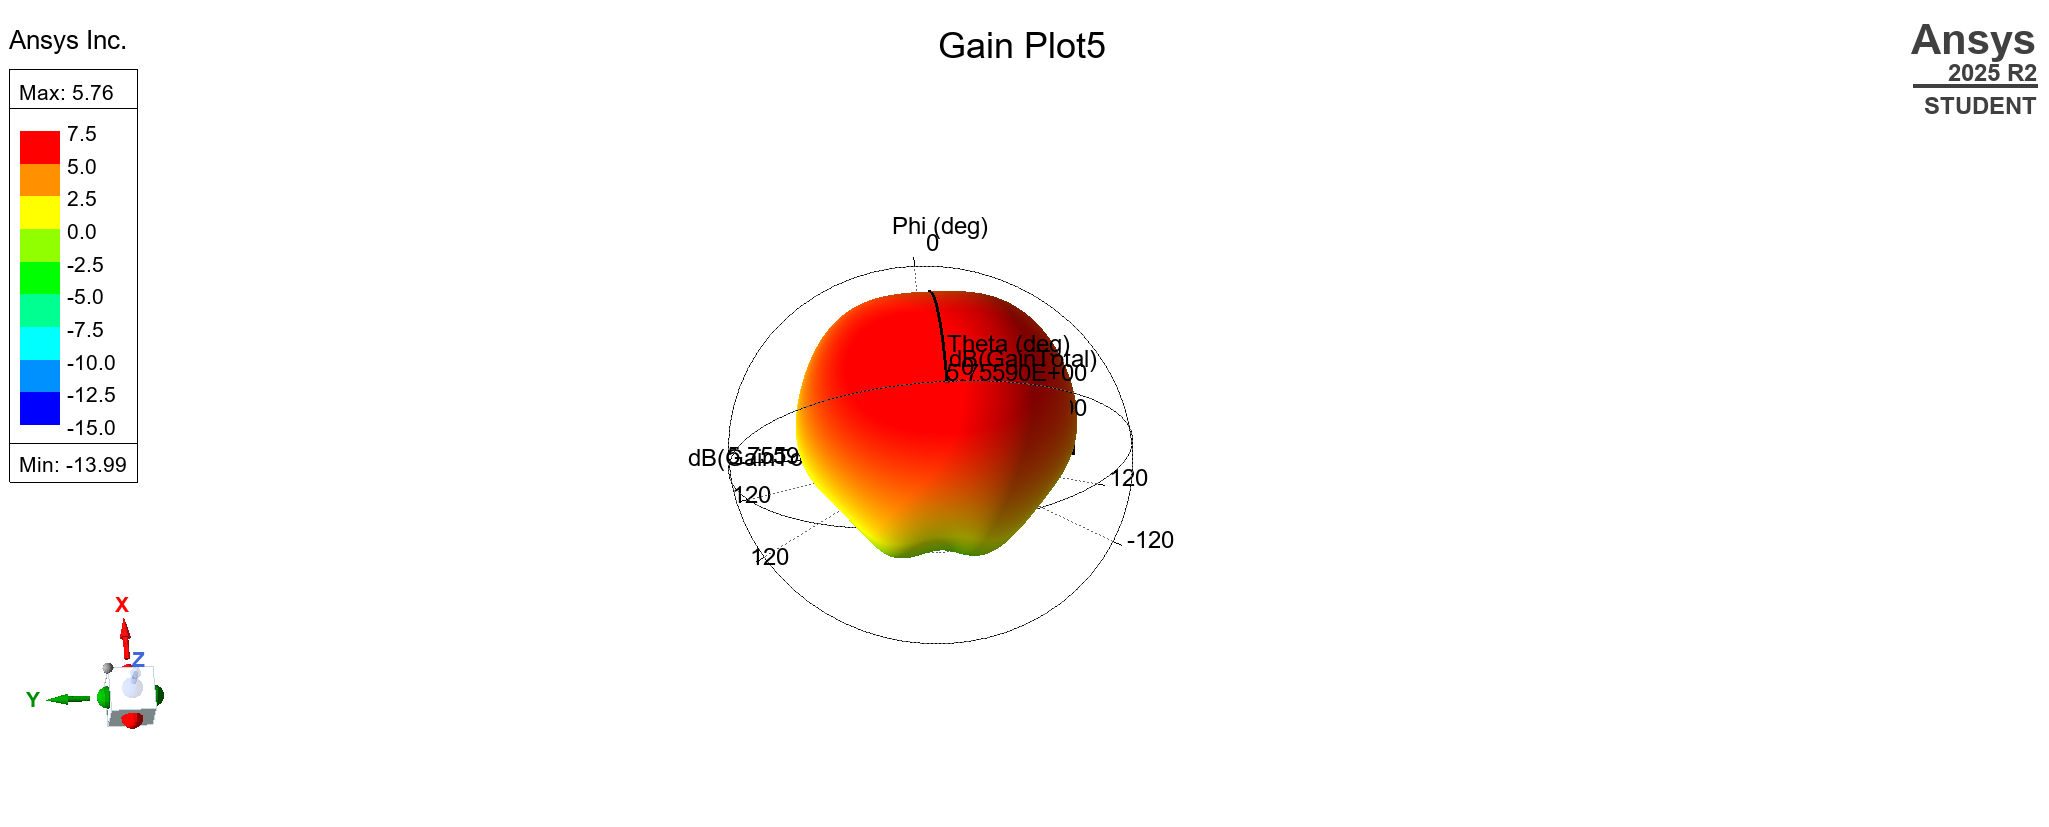
\includegraphics[width=0.9\textwidth]{p32.png}
    \end{minipage}
    \caption{三维方向图}
\end{figure}

【实验结论】：优化 W/L 参数后，天线在新的谐振频率附近保持了良好的定向辐射特性。E 面最大增益为 5.7558 dB，H 面最大增益为 5.7015 dB，与优化前（最大增益 5.81 dB）基本一致。
且此时的谐振频率点位于9.9923GHz，非常接近10GHz目标频率，说明优化后的天线可以在10GHz附近良好工作。
\section{实验总结与实验心得}

\subsection{实验总结}

本次实验围绕 10 GHz 微带贴片天线的设计与仿真展开，通过理论计算、HFSS 建模仿真和参数优化，得到总结如下：

\textbf{理论计算与仿真实践存在差异：}基于经验公式的理论计算（目标 10 GHz）与 HFSS 仿真结果（谐振点 9.7633 GHz）存在约 2.37\% 的偏差。这证实了理论公式的近似性，以及馈线嵌入、切缝等实际结构对天线谐振特性的复杂影响。

\textbf{掌握了 HFSS 仿真全流程：}本实验完整实践了从工程初始化、参数化建模（包括基片、辐射贴片、馈线和切缝）、边界条件（辐射边界）与激励（集总端口）设置，到求解分析与数据后处理的 HFSS 仿真设计全过程。

\textbf{验证了关键参数的调节作用：}实验探究（第 6 节）表明，辐射贴片的长 $L$ 和宽 $W$ 是调节谐振频率的关键参数；而切缝宽度 $d_0$ 主要用于微调阻抗匹配的精细程度。

\textbf{优化实现了设计指标：}通过 W/L 参数的扫参和优化，天线性能得到显著改善。最终在 10 GHz 目标频率下获得了 -25.47 dB 的良好回波损耗和接近 50 $\Omega$ 的输入阻抗，同时保持了约 5.76 dB 的稳定增益，成功达到了设计目标。

\subsection{实验心得}

通过本次实验，我收获良多，心得体会主要有以下三点：

{\heiti 理论是设计的起点，仿真是实践的桥梁。}{ 实验伊始，我严格按照课本中的经验公式（如第 2 节所用）计算初始参数。}但仿真结果（第 4 节）立刻显示理论与实际存在偏差（频率偏低）。这使我深刻认识到，理论公式是理想化模型，它无法精确描述馈线嵌入、切缝乃至有限介质基板带来的边缘效应和电抗加载。HFSS 这样的全波仿真软件弥补了这一点，它让我们能"看见"电磁场，但也必须依赖理论计算给出一个合理的初始值。真正的天线设计，就是在"理论估算"到"仿真验证"，再到"参数调优"的迭代循环中逐步逼近目标的过程。

{\heiti "参数化"是高效仿真的核心。}{ 在第 3 节建模时，报告详细定义了 $W$, $L$, $h$, $y_0$, $d_0$ 等变量。}起初我认为这有些繁琐，但在进行第 6 节的实验探究时，我才体会到参数化建模的巨大优势。当需要调整贴片尺寸或切缝宽度时，我无需重新绘制，只需在变量表中修改数值即可启动扫参（Sweep）或优化（Optimization）。这种"参数化"思想是 HFSS 仿真的精髓，它将重复的机械劳动交给了计算机，让设计者能专注于分析参数变化对结果（如 $S_{11}$ 和频率）的影响。

{\heiti 设计优化是一个系统性的分析过程。}{当初始仿真频率不准时，我面临的问题是：该调哪个参数？}第 6 节的探究给了我答案。我首先尝试了 $d_0$ 扫参，发现它对谐振频率影响不大，但能显著改变 $S_{11}$ 的深度。接着我尝试了 W/L 扫参，发现它们是调节谐振频率的决定性因素。这个过程让我领会到，工程优化不是盲目试错，而是要系统地（methodical）分析每个变量的作用。通过 W/L 修正频率、再（如果需要）通过 $d_0$ 或 $y_0$ 微调匹配，这种"解耦"的思维方式，是本次实验中比仿真结果本身更宝贵的收获。

\end{document}
